\documentclass[10pt,a4paper]{article}
\usepackage[UTF8,fontset = windows]{ctex}
\setCJKmainfont[BoldFont=黑体,ItalicFont=楷体]{华文中宋}
\usepackage{amssymb,amsmath,amsfonts,amsthm,mathrsfs,dsfont,graphicx}
\usepackage{ifthen,indentfirst,enumerate,color,titletoc}
\usepackage{tikz}
\usepackage{makecell}
\usepackage{longtable}
%\usepackage{mathptmx}

\usetikzlibrary{arrows,calc,intersections,patterns,decorations.pathreplacing,3d,angles}
\usepackage[bf,small,indentafter,pagestyles]{titlesec}
\usepackage[top=1in, bottom=1in,left=0.8in,right=0.8in]{geometry}
\renewcommand{\baselinestretch}{1.65}
\newtheorem{defi}{定义~}
\newtheorem{eg}{例~}
\newtheorem{ex}{~}
\newtheorem{rem}{注~}
\newtheorem{thm}{定理~}
\newtheorem{coro}{推论~}
\newtheorem{axiom}{公理~}
\newtheorem{prop}{性质~}
\newcommand{\blank}[1]{\underline{\hbox to #1pt{}}}
\newcommand{\bracket}[1]{(\hbox to #1pt{})}
\newcommand{\onech}[4]{\par\begin{tabular}{p{.9\textwidth}}
A.~#1\\
B.~#2\\
C.~#3\\
D.~#4
\end{tabular}}
\newcommand{\twoch}[4]{\par\begin{tabular}{p{.46\textwidth}p{.46\textwidth}}
A.~#1& B.~#2\\
C.~#3& D.~#4
\end{tabular}}
\newcommand{\vartwoch}[4]{\par\begin{tabular}{p{.46\textwidth}p{.46\textwidth}}
(1)~#1& (2)~#2\\
(3)~#3& (4)~#4
\end{tabular}}
\newcommand{\fourch}[4]{\par\begin{tabular}{p{.23\textwidth}p{.23\textwidth}p{.23\textwidth}p{.23\textwidth}}
A.~#1 &B.~#2& C.~#3& D.~#4
\end{tabular}}
\newcommand{\varfourch}[4]{\par\begin{tabular}{p{.23\textwidth}p{.23\textwidth}p{.23\textwidth}p{.23\textwidth}}
(1)~#1 &(2)~#2& (3)~#3& (4)~#4
\end{tabular}}
\begin{document}
\begin{enumerate}[1.]



\item ``变''角.
所谓变角, 就是将角度进行恒等变换, 为解题作铺垫, 常用的变角类型有$2\alpha =(\alpha +\beta)+(\alpha -\beta)$, $2\beta =(\alpha +\beta)+(\alpha -\beta)$, $\alpha =(\alpha +\beta)-\beta$, $\alpha =(\alpha +45^\circ)-45^\circ$, $\alpha =(m+1)\alpha -m\alpha$, 等等.
\item 已知$\cos (\alpha +\beta)=\dfrac 45$, $\cos (\alpha -\beta)=-\dfrac 45$, 其中$\alpha +\beta \in (\dfrac{7\pi}4,2\pi)$, $\alpha -\beta \in (\dfrac{3\pi}4,\pi)$, 求$\cos 2\alpha$.
解  ' $\because \dfrac{7\pi}4<\alpha +\beta <2\pi$, $\dfrac{3\pi}4<\alpha -\beta <\pi$, $\therefore \sin (\alpha +\beta)=-\dfrac 35$, $\sin (\alpha -\beta)=\dfrac 35$,
于是$\cos 2\alpha =\cos [(\alpha +\beta)+(\alpha -\beta)]=\cos (\alpha +\beta)\cos (\alpha -\beta)-\sin (\alpha +\beta)\sin (\alpha -\beta)$
\blank{50}$=\dfrac 45(-\dfrac 45)-(-\dfrac 35)\times \dfrac 35=-\dfrac{16}{25}+\dfrac 9{25}=-\dfrac 7{25}$.
\item 求证: $\tan (\alpha -\beta)+\tan (\beta -\gamma)+\tan (\gamma -\alpha)=\tan (\alpha -\beta)\tan (\beta -\gamma)\tan (\gamma -\alpha)$.
证明  $\tan (\gamma -\alpha)=-\tan (\alpha -\gamma)=-\tan [(\alpha -\beta)+(\beta -\gamma)]$
\blank{50}$=-\dfrac{\tan (\alpha -\beta)+\tan (\beta -\gamma)}{1-\tan (\alpha -\beta)\tan (\beta -\gamma)}$.
去分母, 得$-\tan (\gamma -\alpha)+\tan (\gamma -\alpha)\tan (\alpha -\beta)\tan (\beta -\gamma)=\tan (\alpha -\beta)+\tan (\beta -\gamma)$,
即$\tan (\alpha -\beta)+\tan (\beta -\gamma)+\tan (\gamma -\alpha)=\tan (\alpha -\beta)\tan (\beta -\gamma)\tan (\gamma -\alpha)$.
\item ``拆''角.
所谓拆角, 就是把已知的角一拆为二, 以达到消项的目的.实际上, 拆角是变角的特例.
\item 求$\dfrac{2\cos 10^\circ -\sin 20^\circ}{\cos 20^\circ}$的值.
解  原试$=\dfrac{2\cos (30^\circ -20^\circ)-\sin 20^\circ}{\cos 20^\circ}=\dfrac{2(\cos 30^\circ \cos 20^\circ +\sin 30^\circ \sin 20^\circ)-\sin 20^\circ}{\cos 20^\circ}$
\blank{50}$=\dfrac{2\cos 30^\circ \cos 20^\circ}{\cos 20^\circ}=\sqrt 3$.
注意  上述解法是把10°``拆''成$30^\circ -20^\circ$来求解, 如果把20°``拆''成$30^\circ -10^\circ$也可获解, 但过程较冗赘.
\item 正、余互变.
如果$\alpha +\beta =\dfrac{\pi}2$, 那么$\sin \alpha =\cos \beta$, $\cos \alpha =\sin \beta$, $\tan \beta =\cot \alpha$.例如, 由$(\dfrac{\pi}3-\varphi)+(\dfrac{\pi}6+\varphi)=\dfrac{\pi}2$, 可得$\sin (\dfrac{\pi}3-\varphi)=\cos (\dfrac{\pi}6+\varphi)$.
\item 已知$\sin (\dfrac{\pi}4-x)=\dfrac 5{13}$, 且$0<x<\dfrac{\pi}4$.求$\dfrac{\cos 2x}{\cos (\dfrac{\pi}4+x)}$的值.
解  由条件, 得$\cos (\dfrac\pi 4-x)=\dfrac {12}{13}$.
$\therefore$原式$=\dfrac{\sin (\dfrac{\pi}2-2x)}{\cos (\dfrac{\pi}4+x)}=\dfrac{\sin 2(\dfrac{\pi}4-x)}{\cos (\dfrac{\pi}4+x)}=\dfrac{2\sin (\dfrac{\pi}4-x)\cos (\dfrac{\pi}4-x)}{\cos (\dfrac{\pi}4+x)}$
\blank{50}$=\dfrac{2\cos (\dfrac\pi 4+x)\cos (\dfrac{\pi}4-x)}{\cos (\dfrac{\pi}4+x)}=2\cos (\dfrac{\pi}4-x)=\dfrac {24}{13}$.
\item 逆用公式.
由$\tan (\alpha +\beta)=\dfrac{\tan \alpha +\tan \beta}{1-\tan \alpha \tan \beta}$可得
$\tan \alpha +\tan \beta =\tan (\alpha +\beta)(1-\tan \alpha \tan \beta)$, 或$1-\tan \alpha \tan \beta =\dfrac{\tan \alpha +\tan \beta}{\tan (\alpha +\beta)}$.
后两个公式是第一个公式的逆用.
\item 求$\tan 65^\circ +\tan 70^\circ +1-\tan 65^\circ \tan 70^\circ$的值.
解  原式$=\tan (65^\circ +70^\circ)(1-\tan 65^\circ \tan 70^\circ)+1-\tan 65^\circ \tan 70^\circ$
\blank{50}$=(-1)\cdot (1-\tan 65^\circ \tan 70^\circ)+1-\tan 65^\circ \tan 70^\circ =0$.
注意  此例也可用``他推法''求解.所谓``他推法'', 即从某已知等式出发, 经过变换后, 便可获得欲求之解.
如例5, $\because 135^\circ =65^\circ +70^\circ$, 两边取正切, 便得$-1=\tan (65^\circ +70^\circ)=\dfrac{\tan 65^\circ +\tan 70^\circ}{1-\tan 65^\circ \tan 70^\circ}$,
$\therefore \tan 65^\circ \tan 70^\circ -1=\tan 65^\circ +\tan 70^\circ$, 移项即可得原式$=0$.
请读者思考, 如何通过``公式逆用''或``他推法''来证明:
$\tan (A-B)+\tan (B-C)+\tan (C-A)=\tan (A-B)\tan (B-C)\tan (C-A)$.
\item 合一变形.
形如$a\sin x+b\sin x$的式子颇为常见.此类式子可作``合一变形'', 即
$a\sin x+b\sin x=\sqrt {a^2+b^2}(\dfrac a{\sqrt {a^2+b^2}}\sin x+\dfrac b{\sqrt {a^2+b^2}}\cos x)=\sqrt {a^2+b^2}\sin (x+\varphi)$,
其中, $\sin \varphi =\dfrac b{\sqrt {a^2+b^2}}$, $\cos \varphi =\dfrac a{\sqrt {a^2+b^2}}$.
由此便可求得$a\sin x+b\sin x$的值域、周期和单调区间等.
\item 求函数$f(x)=\sin x-\sqrt 3\cos x$的值域、最小正周期以及为增函数的区间.
解  $\because f(x)=2(\sin x\cdot \dfrac 12-\cos x\cdot \dfrac{\sqrt 3}2)=2\sin (x-\dfrac{\pi}3)$,
$\therefore$函数的值域为[-2, 2], 最小正周期是$2\pi$, 为增函数的区间是$[2k\pi -\dfrac{\pi}6,2k\pi +\dfrac{5\pi}6]$($k\in \mathbf{Z}$).
\item 求函数$y=\dfrac{\sqrt 3\sin x}{2+\cos x}$的值域.
解  由已知, 得$2y+y\cos x=\sqrt 3\sin x$, 即$\sqrt 3\sin x-y\cos x=2y$,
$\therefore \sin x\cdot \dfrac{\sqrt 3}{\sqrt {3+y^2}}-\cos x\cdot \dfrac y{\sqrt {3+y^2}}=\dfrac{2y}{\sqrt {3+y^2}}$.
于是$\sin (x-\varphi)=\dfrac{2y}{\sqrt {3+y^2}}$(其中$\varphi$满足$\sin \varphi =\dfrac y{\sqrt {3+y^2}}$, $\cos \varphi =\dfrac{\sqrt 3}{\sqrt {3+y^2}}$).
$\because|\sin (x-\varphi)|\le 1$, $\therefore \dfrac{2y}{\sqrt {3+y^2}}\le 1$, $\therefore -1\le y\le 1$.
注意  对于求$y=\dfrac{a\sin x+b\cos x+c}{a'\sin x+b'\cos x+c'}$的值域, 均可采用例7的方法, 即去分母, 合一变形, 解不等式三个步骤.
\item 升幂和降幂.
(1)升幂.运用公式$1+\cos 2x=2\cos ^2x$, $1-\cos 2x=2\sin ^2x$.
\item 化简$\dfrac{1+\cos \theta -\sin \theta}{1-\cos \theta -\sin \theta}+\dfrac{1-\cos \theta -\sin \theta}{1+\cos \theta -\sin \theta}$.
解  原式$=\dfrac{2\cos ^2\dfrac{\theta}2-2\sin \dfrac{\theta}2\cos \dfrac{\theta}2}{2\sin ^2\dfrac{\theta}2-2\sin \dfrac{\theta}2\cos \dfrac{\theta}2}+\dfrac{2\sin ^2\dfrac{\theta}2-2\sin \dfrac{\theta}2\cos \dfrac{\theta}2}{2\cos ^2\dfrac{\theta}2-2\sin \dfrac{\theta}2\cos \dfrac{\theta}2}$
\blank{50}$\begin{cases} =\dfrac{\cos \dfrac{\theta}2(\cos \dfrac{\theta}2-\sin \dfrac{\theta}2)}{\sin \dfrac{\theta}2(\sin \dfrac{\theta}2-\cos \dfrac{\theta}2)}+\dfrac{\sin \dfrac{\theta}2(\sin \dfrac{\theta}2-\cos \dfrac{\theta}2)}{\cos \dfrac{\theta}2(\cos \dfrac{\theta}2-\sin \dfrac{\theta}2)} \\ =-(\cot \dfrac\theta 2+\tan \dfrac{\theta}2)=-(\dfrac {1+\cos \theta}{\sin \theta}+\dfrac{1-\cos \theta}{\sin \theta})=-\dfrac 2{\sin \theta}=-2\csc \theta . \end{cases}$
(2)降幕.逆用公式$\cos 2\alpha =2\cos ^2\alpha -1$和$\cos 2\alpha =1-2\sin ^2\alpha$,
可得$\cos ^2\alpha =\dfrac{1+\cos 2\alpha}2$, $\sin ^2\alpha =\dfrac{1-\cos 2\alpha}2$.
\item 求函数$y=3\sin ^2\alpha -4\sin \alpha \cdot \cos \alpha +\cos ^2\alpha$的值域和最小正周期.
解  $\because y=3\cdot \dfrac{1-\cos 2\alpha}2-2\sin 2\alpha +\dfrac{1+\cos 2\alpha}2=2-(2\sin 2\alpha +\cos 2\alpha)=2-\sqrt 5(2\alpha +\varphi)$,
其中$\sin \varphi =\dfrac 1{\sqrt 5}$, $\cos \varphi =\dfrac 2{\sqrt 5}$, $\therefore$函数的值域是$[2-\sqrt 5,2+\sqrt 5]$, 最小正周期是$\pi$.
注意  对于形如$y=a\sin ^2\alpha +b\sin \alpha \cos \alpha +c\cos ^2\alpha$的函数, 宜采用``先降幂, 后合一''的方法进行化简, 再研究其性质.
【训练题】
(一)两角和(差)的余弦公式
\item 化简$\sin (x+y)\sin x+\cos (x+y)\cos x$的结果是()
\fourch{$\cos (2x+y)$}{$\cos y$}{$\sin (2x+y)$}{$\sin y$}
\item 满足$\cos \alpha \cos \beta =\dfrac{\sqrt 3}2+\sin \alpha \sin \beta$的一组$\alpha ,\beta$的值是()
\fourch{$\alpha =\dfrac{13\pi}{12},\beta =\dfrac{3\pi}4$}{$\alpha =\dfrac{\pi}2,\beta =\dfrac{\pi}3$}{$\alpha =\dfrac{\pi}2,\beta =\dfrac{\pi}6$}{$\alpha =\dfrac{\pi}3,\beta =\dfrac{\pi}6$}
\item 若$\dfrac{3\pi}2<\alpha <2\pi$, 且$\cot (\dfrac{3\pi}2+\alpha)=\dfrac 34$, 则$\cos (\alpha -\dfrac{3\pi}2)$的值等于()
\fourch{$\dfrac{\sqrt 2}{10}$}{$-\dfrac{\sqrt 2}{10}$}{$\dfrac{7\sqrt 2}{10}$}{$-\dfrac{7\sqrt 2}{10}$}
\item 若三角形的两内角$\alpha ,\beta$满足$\cos \alpha \cos \beta >\sin \alpha \sin \beta$, 则这个三角形的形状()
\fourch{是锐角三角形}{是貞角三角形}{是钝角三角形}{不能确定}
\item 若关于$x$的方程$x^2+x\cos \alpha \cos \beta +\cos \gamma =0$的两根$x_1,x_2$满足$x_1+x_2=\dfrac{x_1x_2}2$, 则以$\alpha ,\beta ,\gamma$为内角的三角形的形状()
\fourch{是等腰三角形, 不可能是直角三角形}{是直角三角形, 不可能是等腰三角形}{是等腰直角三角形}{是等腰三角形, 也可能是直角三角形}
\item (1)若$\tan x=\dfrac 43$($\pi <x<2\pi$), 则$\cos (2x-\dfrac{\pi}3)\cdot \cos (\dfrac{\pi}3-x)-\sin (2x-\dfrac{\pi}3)\cdot \sin (\dfrac{\pi}3-x)=$\blank{50}.
(2)若锐角$\alpha ,\beta$满足$\cos \alpha =\dfrac 35$, $\cos (\alpha +\beta)=-\dfrac 5{13}$则$\cos \beta =$\blank{50}.
(3)若$\cos (\alpha -\beta)=-\dfrac 45$, $\cos (\alpha +\beta)=\dfrac 45$, 且$90^\circ <\alpha -\beta <180^\circ$, $270^\circ <\alpha +\beta <360^\circ$, 则$\cos 2\alpha =$\blank{50}, $\cos 2\beta =$\blank{50}.
(4)若$\cos x+\cos y=\dfrac 12$, $\sin x-\sin y=\dfrac 13$, 则$\cos (x+y)=$\blank{50}.
\item 若$\sin \alpha \sin \beta =1$, 则$\cos (\alpha +\beta)$的值是()
\fourch{-1}{0}{1}{$\pm 1$}
\item 若$\alpha ,\beta$为锐角, 则()
\fourch{$\cos (\alpha +\beta)>\cos \alpha +\cos \beta$}{$\cos (\alpha +\beta)>\sin \alpha +\sin \beta$}{$\cos (\alpha +\beta)<\cos \alpha +\cos \beta$}{$\cos (\alpha +\beta)<\sin \alpha +\sin \beta$}
\item 若$\sin \alpha +\sin \beta =\dfrac{\sqrt 2}2$, 则$\cos \alpha +\cos \beta$的取值范围是()
\fourch{$[0,\dfrac{\sqrt 2}2]$}{$[-\dfrac{\sqrt 2}2,\dfrac{\sqrt 2}2]$}{[―2, 2]}{$[-\dfrac{\sqrt {14}}2,\dfrac{\sqrt {14}}2]$.}
\item 若三角形的两内角$\alpha ,\beta$满足$\tan \alpha \tan \beta >1$, 则这个三角形的形状是()
\fourch{等腰直角三角形}{不等腰的直角三角形}{锐角三角形}{钝角三角形}
\item 若三角形的两内角$\alpha ,\beta$满足$\sin \alpha =\dfrac 35$, $\cos \beta =\dfrac 5{13}$, 则此三角形的另—内角$\gamma$的余弦值等于()
\fourch{$\dfrac{16}{65}$或$\dfrac{56}{65}$}{$\dfrac{56}{65}$}{$\dfrac{16}{65}$}{$-\dfrac{16}{65}$或$-\dfrac{56}{65}$}
\item (1)已知锐角$\alpha ,\beta$满足$\cos \alpha =\dfrac 45$, $\tan (\alpha -\beta)=-\dfrac 13$, 求$\cos \beta$.
(2)已知$\cos (\dfrac{\pi}4-\alpha)=\dfrac 35$, $\sin (\dfrac{3\pi}4+\beta)=\dfrac 5{13}$, 其中$\dfrac{\pi}4<\alpha <\dfrac{3\pi}4$, $0<\beta <\dfrac{\pi}4$, 求$\sin (\alpha +\beta)$的值.
(3)已知$\alpha ,\beta$为锐角, 满足$\cos \alpha =\dfrac 17$, $\sin (\alpha +\beta)=\dfrac{5\sqrt 3}{14}$, 求$\cos \beta$的值.
\item 已知$8\cos (2\alpha +\beta)+5\cos \beta =0$, 求$\tan (\alpha +\beta)\cdot \tan \alpha$的值.
\item 解不等式: $\sin 4x+\cos 4x\cdot \cot 2x>1$.
\item 已知锐角$\alpha ,\beta ,\gamma$满足$\sin \alpha +\sin \gamma =\sin \beta$, $\cos \alpha -\cos \gamma =\cos \beta$, 求$\alpha -\beta$的值.
(二)两角和(差)的正弦公式
\item 若$\alpha ,\beta$为锐角, 且满足$\cos \alpha =\dfrac 45$, $\cos (\alpha +\beta)=\dfrac 35$, 则$\sin \beta$的值是()
\fourch{$\dfrac{17}{25}$}{$\dfrac 35$}{$\dfrac 7{25}$}{$\dfrac 15$}
\item 函数$y=\sin (x+\dfrac{\pi}3)-\sqrt 3\cos (x+\dfrac{\pi}3)$()
\fourch{是奇函数, 但不是偶函数}{是偶函数, 但不是奇函数}{既不是奇函数, 也不是偶函数}{奇偶性无法确定}
\item 下列函数中, 与$y=\sin x+\cos x$的振幅、最小正周期都相同的函数是()
\fourch{$y=\sin x$}{$y=\cos x$}{$y=\sqrt 2\sin x$}{$y=\sin x\cos x$}
\item 函数$y=\sin x+\sqrt 3\cos x$($0\le x\le \dfrac{\pi}2$)的值域是()
\fourch{$[1,\dfrac 32]$}{[1, 2]}{$[\dfrac 32,2]$}{[0, 2]}
\item (1)化简$\sin (x+27^\circ)\cos (18^\circ -x)+\cos (x+27^\circ)\sin (18^\circ -x)=$\blank{50}.
(2)函数$y=3\sin 2x+3\sqrt 3\cos 2x+1$的最小正周期是\blank{50}, 最大值是\blank{50}, 最小值是\blank{50}.
\item 若$\alpha$是一个三角形的最小内角, 则函数$y=\sin \alpha -\cos \alpha$的值域为()
\fourch{$[-\sqrt 2,\sqrt 2]$}{$(-1,\dfrac{\sqrt 3-1}2)$}{$(-1,\dfrac{\sqrt 3-1}2]$}{$[-1,\dfrac{\sqrt 3-1}2]$}
\item 若函数$f(x)=\sin 2x+a\cos 2x$的图像关于直线$x=-\dfrac{\pi}8$对称, 则实数$a$的值等于()
\fourch{$\sqrt 2$}{$-\sqrt 2$}{1}{-1}
\item (1)若以$\sin (45^\circ -\alpha)=-\dfrac 23$, $\dfrac{\pi}4<\alpha <\dfrac{\pi}2$, 则$\sin \alpha =$\blank{50}.
(2)计算: $\dfrac{\sin 7^\circ +\sin 8^\circ \cos 15^\circ}{\cos 7^\circ -\sin 8^\circ \sin 15^\circ}=$\blank{50}.
(3)计算: $\csc 10^\circ -\sqrt 3\sec 10^\circ =$\blank{50}.
\item (1)函数$y=\log _{0.2}(\sin x+\cos x)$为增函数的区间是\blank{50}.
(2)不等式$\sin x<\cos x$的解是\blank{50}.
\item 求下列函数的值域:
(1)$y=\dfrac{\sqrt 5\sin x+1}{\cos x+2}$.					(2)$y=\dfrac{\tan \theta +2}{\sec \theta -1}$.
\item 在$\triangle ABC$中, 已知$2\cos B\cos C=1-\cos A$, 且$2\sin B\cos C=1+\sin (B-C)$, 判断此三角形的形状.
\item (1)已知关于$x$的方程$x^2+px+q=0$的两根是$\tan \alpha$, $\tan \beta$, 求$\dfrac{\sin (\alpha +\beta)}{\cos (\alpha -\beta)}$的值.
(2)已知$\sin (\alpha +\beta)=\dfrac 12$, $\sin (\alpha -\beta)=\dfrac 13$, 求$\tan \alpha \cot \beta$的值.
(3)已知$\tan (\alpha +\beta)=-2$, $\tan (\alpha -\beta)=\dfrac 12$, 求$\dfrac{\sin 2\alpha}{\sin 2\beta}$的值.
\item 已知$\tan \alpha =1$, $3\sin \beta =\sin (2\alpha +\beta)$, 求$\tan (\alpha +\beta)$的值.
29已知$\dfrac{\tan (\alpha -\gamma)}{\tan \alpha}+\dfrac{\sin ^2\beta}{\sin ^2\alpha}=1$, 求证: $\tan ^2\beta =\tan \alpha \tan \gamma$.
\item (1)求函数$y=\dfrac{\sin x\cos x}{1+\sin x+\cos x}$的最大值,
(2)求函数$y=\sin x+\cos x+\sin x\cos x$的值域.
(3)$a\in \mathbf{R}$, 求$y=(\sin x+a)(\cos x+a)$的最小值.
注意  对于含$\sin x\pm \cos x$, $\sin x\cos x$的三角函数式, 可令$t=\sin x\pm \cos x$, 则$\sin x\cos x=\pm \dfrac{t^2-1}2$, $t\in [-\sqrt 2,\sqrt 2]$.
(三)两角和(差)的正切公式
\item 若$\tan (\alpha +\beta)=\dfrac 25$, $\tan (\beta -\dfrac{\pi}4)=\dfrac 14$, 则$\tan (\alpha +\dfrac{\pi}4)$等于()
\fourch{$\dfrac{13}{18}$}{$\dfrac{13}{22}$}{$\dfrac 3{22}$}{$\dfrac 16$}
\item 若$\dfrac{1-\tan A}{1+\tan A}=4+\sqrt 5$, 则$\cot (\dfrac{\pi}4+A)$的值等于()
\fourch{$-4-\sqrt 5$}{$4+\sqrt 5$}{$-\dfrac 1{4+\sqrt 5}$}{$\dfrac 1{4+\sqrt 5}$}
\item 已知$\alpha +\beta =\dfrac{3\pi}4$, 则$(1-\tan \alpha)(1-\tan \beta)$的值等于()
\fourch{2}{-2}{1}{-1}
\item (1)计算$\dfrac{1+\cot 15^\circ}{1-\tan 75^\circ}=$\blank{50}.
(2)若$\alpha +\beta =\dfrac{\pi}4$, 则$\dfrac{1-\tan \beta}{1+\tan \beta}=$\blank{50}.
(3)若$\tan x=\dfrac 12$, $\tan (x-y)=-\dfrac 25$, 则$\tan (2x-y)=$\blank{50}.
(4)在$\triangle ABC$中, $\tan A$, $\tan B$是方程$3x^2+8x-1=0$的两个根, 则$\tan C=$\blank{50}.
(5)若$\tan (\alpha +\dfrac{\pi}4)=-\dfrac 9{40}$, 则$\tan \alpha =$\blank{50}, $\tan (\alpha -\dfrac{\pi}4)=$\blank{50}.
\item 若$\alpha ,\beta \in (\dfrac{\pi}2,\pi)$, 且$\tan \alpha <\cot \beta$, 则()
\fourch{$\alpha <\beta$}{$\beta >\alpha$}{$\pi <\alpha +\beta <\dfrac{3\pi}2$}{$\alpha +\beta >\dfrac{3\pi}2$}
\item 函数$y=\dfrac{\cos 2x+\sin 2x}{\cos 2x-\sin 2x}$的最小正周期是()
\fourch{$2\pi$}{$\dfrac{3\pi}2$}{$\pi$}{$\dfrac{\pi}2$}
\item 若$-\dfrac{\pi}2<\alpha <\dfrac{\pi}2$, $-\dfrac{\pi}2<\beta <\dfrac{\pi}2$, 且$\tan \alpha$, $\tan \beta$是方程$x^2+3\sqrt 3x+4=0$的两个根, 则$\alpha +\beta$等于()
\fourch{$\dfrac{\pi}3$}{$-\dfrac{2\pi}3$}{$\dfrac{\pi}3$或$\dfrac{4\pi}3$}{$\dfrac{\pi}3$或$-\dfrac{2\pi}3$}
\item (1)若$\tan \theta$和$\tan (\dfrac{\pi}4-\theta)$是方程$x^2+px+q=0$的两个根, 则$p,q$满足关系式\blank{50}.
(2)若$\tan \alpha =\dfrac 17$, $\tan \beta =\dfrac 13$, $0<\alpha ,\beta <\dfrac{\pi}2$, 则$\alpha +2\beta =$\blank{50}.
\item (1)计算: $1+\tan 66^\circ +\tan 69^\circ -\tan 66^\circ \tan 69^\circ =$\blank{50}.
(2)计算: $\tan 19^\circ +\tan 101^\circ -\sqrt 3\tan 19^\circ \tan 101^\circ =$\blank{50}.
(3)若$\alpha +\beta =k\pi +\dfrac{\pi}4$($k\in \mathbf{Z}$), 则$(1+\tan \alpha)(1+\tan \beta)=$\blank{50}.
(4)计算$(1+\tan 1^\circ)(1+\tan 2^\circ)(1+\tan 3^\circ)\cdots (1+\tan 43^\circ)(1+\tan 44^\circ)=$\blank{50}.
\item (1)求证: $\tan 20^\circ \tan 30^\circ +\tan 30^\circ \tan 40^\circ +\tan 40^\circ \tan 20^\circ =1$.
(2)求证: $\tan (A-B)+\tan (B-C)+\tan (C-A)=\tan (A-B)\tan (B-C)\tan (C-A)$.
(3)求证: $\tan A+\tan B+\tan C=\tan A\tan B\tan C$, 其中$A+B+C=k\pi$($k\in \mathbf{Z}$).
\item 已知锐角$\alpha ,\beta$满足$\tan \alpha =\sqrt 3(m+1)$, $\tan (-\beta)=\sqrt 3(\tan \alpha \tan \beta +m)$, 求$\alpha +\beta$的值.
\item (1)求$\dfrac{\tan 20^\circ +\tan 40^\circ +\tan 120^\circ}{\tan 20^\circ \tan 40^\circ}$的值.
(2)已知$\tan \theta =\dfrac{\sin \alpha -\cos \alpha}{\sin \alpha +\cos \alpha}$($\alpha ,\theta$都是锐角), 求$\dfrac{\sin \alpha -\cos \alpha}{\sin \theta}$的值.
(3)已知$\tan (\dfrac{\pi}4+\alpha)=-\dfrac 12$, 求$\dfrac{2\cos \alpha (\sin \alpha -\cos \alpha)}{1+\tan \alpha}$的值.
\item 已知$\tan \alpha$, $\tan \beta$是关于$x$的方程$mx^2-2x\sqrt {7m-3}+2m=0$的两个实根, 求$\tan (\alpha +\beta)$的取值范围.
(四)二倍角的正弦公式
\item 若$\sin \alpha +\cos \alpha =-\sqrt 2$, 则$\tan \alpha +\cot \alpha$等于()
\fourch{-2}{-1}{1}{2}
\item 若三角形的一个内角$\alpha$满足$\sin \alpha +\cos \alpha =\dfrac 34$, 则这个三角形的形状是()
\fourch{锐角三角形}{钝角三角形}{不等腰的直角三角形}{等腰直角三角形}
\item 函数$f(x)=\sqrt {\cos ^2x-\cos ^4x}$的最小正周期为()
\fourch{$\dfrac{\pi}2$}{$\pi$}{$\dfrac{3\pi}2$}{$2\pi$}
\item 若$\alpha \in [\dfrac{5\pi}2,\dfrac 72\pi]$, 则$\sqrt {1+\sin \alpha}+\sqrt {1-\sin \alpha}$的值为()
\fourch{$2\cos \dfrac{\alpha}2$}{$-2\cos \dfrac{\alpha}2$}{$2\sin \dfrac{\alpha}2$}{$-2\sin \dfrac{\alpha}2$}
\item 函数$y=\log _{0.5}(\sin x\cos x)$为增函数的区间是()
\fourch{$(k\pi -\dfrac{\pi}4,k\pi +\dfrac{\pi}4)$($k\in \mathbf{Z}$)}{$(k\pi ,k\pi +\dfrac{\pi}4]$($k\in \mathbf{Z}$)}{$(k\pi +\dfrac{\pi}4,k\pi +\dfrac{\pi}2)$($k\in \mathbf{Z}$)}{$[k\pi +\dfrac{\pi}4,k\pi +\dfrac{3\pi}4)$($k\in \mathbf{Z}$)}
\item $\cos \dfrac{\pi}5\cos \dfrac{2\pi}5$的值等于()
\fourch{4}{$\dfrac 14$}{2}{$\dfrac 12$}
\item (1)若$\cos ^2(\dfrac x2)=\sin x$, 则$\tan \dfrac x2$等于\blank{50}.
(2)计算: \textcircled{1} $\sin 105^\circ \cos 75^\circ =$\blank{50};
\textcircled{2} $\cos ^215^\circ +\cos ^275^\circ +\cos 15^\circ \cos 75^\circ =$\blank{50};
\textcircled{3} $\cos \dfrac{5\pi}8\cos \dfrac{\pi}8=$\blank{50}.
(3)函数$y=\cos (\dfrac{\pi}2x)\cos [\dfrac{\pi}2(x-1)]$的最小正周期是\blank{50}.
(4)若$\sin x-\cos x=\dfrac 12$, 则$\sin ^3x-\cos ^3x=$\blank{50}.
\item (1)在$\triangle ABC$中, $\angle C=90^{\circ}$, $\tan A+\tan B=4$, 则此三角形的两个锐角分別等于\blank{50}.
(2)若$\sin 2\alpha =\dfrac 45$, 则$\tan ^2\alpha +\cot ^2\alpha =$\blank{50}.
\item 若$\sin x\cos y=\dfrac 12$, 则$\cos x\sin y$的取值范围是()
\fourch{$[-\dfrac 12,\dfrac 12]$}{$[-\dfrac 32,\dfrac 12]$}{$[-\dfrac 12,\dfrac 32]$}{$[-1,1]$}
\item 求值:
(1)$\sin 18^\circ \sin 54^\circ$.						(2)$\cos \dfrac{\pi}{17}\cos \dfrac{2\pi}{17}\cos \dfrac{4\pi}{17}\cos \dfrac{8\pi}{17}$.
\item 求值:
(1)$\cos ^4(\dfrac{\pi}8)+\cos ^4(\dfrac{3\pi}8)+\cos ^4(\dfrac{5\pi}8)+\cos ^4(\dfrac{7\pi}8)$.
(2)$\sin ^4(\dfrac{\pi}{16})+\sin ^4(\dfrac{3\pi}{16})+\sin ^4(\dfrac{5\pi}{16})+\sin ^4(\dfrac{7\pi}{16})$.
\item 求值:
(1)$\csc 10^\circ -\sqrt 3\sec 10^\circ$.					(2)$\cos 40^\circ (1+\sqrt 3\cot 80^\circ)$.
(3)$\tan 70^\circ \cos 10^\circ (\sqrt 3\tan 20^\circ -1)$.		(4)$\sec 50^\circ +\cot 80^\circ$.
(五)二倍角的余弦公式
\item 若$x=\dfrac{\pi}{12}$, 则$\cos ^4x-\sin ^4x$的值为()
\fourch{0}{$\dfrac 12$}{$\dfrac{\sqrt 2}2$}{$\dfrac{\sqrt 3}2$}
\item 函数$y=\sin ^2x$是(),
\fourch{最小正周期为$2\pi$的偶函数}{最小正周期为$2\pi$的奇函数}{最小正周期为$\pi$的偶函数}{最小正周期为$\pi$的奇函数}
\item 若$\sin \dfrac{\alpha}2=\dfrac 35$, $\cos \dfrac{\alpha}2=-\dfrac 45$, 则角$\alpha$所在的象限是()
\fourch{第一象限}{第二象限}{第三象限}{第四象限}
\item 函数$y=2\sin x\cos sx-(\cos ^2x-\sin ^2x)$的最大值与最小值之积等于()
\fourch{2}{-2}{1}{-1}
\item 函数$y=1-\cos ^2x+\cos ^4x$的最小正周期是()
\fourch{$2\pi$}{$\pi$}{$\dfrac{\pi}2$}{$\dfrac{\pi}4$}
\item 化简$\sqrt {1-\cos 4-\sin ^22}$的结果是()
\fourch{$\cos 2$}{$-\cos 2$}{$\sqrt 3\cos 2$}{$-\sqrt 3\cos 2$}
\item (1)若$\sin \theta :\sin \dfrac{\theta}2=8:5$, 则$\cos \theta =$\blank{50}.
(2)计算$\sin \dfrac{\pi}8\cos \dfrac{\pi}8\cot \dfrac{\pi}8=$\blank{50}.
(3)若$8\cos (\dfrac{\pi}8+\alpha)\cos (\dfrac{\pi}4-\alpha)=1$, 则$\sin ^4\alpha +\cos ^4\alpha =$\blank{50}.
(4)函数$y=\sin x\cos x-2\sin ^3x\cos x$的最小正周期是\blank{50}.
(5)若$\tan x=\sqrt 2$, 则$\dfrac{2\cos ^2\dfrac x2-\sin x-1}{\sin x+\cos x}=$\blank{50}.
(6)函数$y=2\sin x(\sin x+\cos x)$为减函数的区间是\blank{50}.
\item 若$270^\circ <\alpha <360^\circ$, 则化简$\sqrt {\dfrac 12+\dfrac 12\sqrt {\dfrac 12+\dfrac 12\cos 2\alpha}}$的结果是()
\fourch{$\sin \dfrac{\alpha}2$}{$-\sin \dfrac{\alpha}2$}{$\cos \dfrac{\alpha}2$}{$-\cos \dfrac{\alpha}2$}
\item 若$\pi <x<\dfrac{3\pi}2$, 则$\sqrt {\tan x+\sin x}+\sqrt {\tan x-\sin x}$可以化成()
\fourch{$2\sqrt {\tan x}\sin (\dfrac x2-\dfrac{\pi}4)$}{$2\sqrt {\tan x}\sin (\dfrac x2+\dfrac{\pi}4)$}{$-2\sqrt {\tan x}\sin (\dfrac x2-\dfrac{\pi}4)$}{$-2\sqrt {\tan x}\sin (\dfrac x2+\dfrac{\pi}4)$}
\item (1)已知$\sin \alpha +\sin \beta =\dfrac 12$, $\cos \alpha +\cos \beta =\dfrac 13$, 求$\cos ^2(\dfrac{\alpha -\beta}2)$的值.
(2)求$y=\sin ^6x+\cos ^6x$的最小正周期.
(3)已知$\tan \alpha \tan \beta =\dfrac 1{\sqrt 3}$, 求$(2-\cos 2\alpha)(2-\cos 2\beta)$的值.
\item (1)化简: $\dfrac{2\cos ^2\alpha -1}{2\tan (\dfrac{\pi}4-\alpha)\sin ^2(\dfrac{\pi}4+\alpha)}$.(2)化简: $\dfrac{1+\cos \theta -\sin \theta}{1-\cos \theta -\sin \theta}+\dfrac{1-\cos \theta -\sin \theta}{1+\cos \theta -\sin \theta}$.
(3)已知$\cos (\dfrac{\pi}4+x)=\dfrac 45$($\dfrac{19\pi}{12}<x<\dfrac{7\pi}4$), 求$\dfrac{\sin 2x-2\sin ^2x}{1-\tan x}$的值.
\item 求下列函数的最大值及其相成的$x$值:
(1)$f(x)=4\cos 2x+12\sin x-5\cos ^2x$.	(2)$f(x)=\sin 2x+\sin x+\cos x$.
(3)$f(x)=\dfrac{\sin x\cos x}{1+\sin x+\cos x}$.
\item 求函数$y=\sin ^2x+2\sin x\cos x+3\cos ^2x-2$的取值范、最小正周期以及为增函数的区间.
(六)万能公式
\item 化简$\dfrac{\cot \dfrac{\alpha}2-\tan \dfrac{\alpha}2}{\cot \dfrac{\alpha}2+\tan \dfrac{\alpha}2}$的结果是()
\fourch{$\sin \alpha$}{$\cos \alpha$}{$\tan \alpha$}{$\cot \alpha$}
\item 函数$y=\lg \dfrac{\tan x}{1+\tan x}$为增函数的区间是()
\fourch{$(k\pi ,k\pi +\dfrac{\pi}4]$, $k\in \mathbf{Z}$}{$(k\pi ,2k\pi +\dfrac{\pi}4]$, $k\in \mathbf{Z}$}{$(2k\pi ,2k\pi +\dfrac{\pi}2]$, $k\in \mathbf{Z}$}{$(2k\pi ,k\pi +\dfrac{\pi}2]$, $k\in \mathbf{Z}$}
\item 若$f(\tan x)=\sin 2x$, 则$f(-1)$的値是()
\fourch{$-\sin 2$}{-1}{$\dfrac 12$}{1}
\item 若$\tan \dfrac A2=\dfrac mn$, 则$m\cos A-n\sin A$等于()
\fourch{$n$}{$-n$}{$m$}{$-m$}
\item 若锐角$\theta$满足$\sin \dfrac\theta 2=\sqrt {\dfrac {x-1}{2x}}$, 则$\tan \theta$等于()
\fourch{$x$}{$\dfrac{x+1}{\sqrt {x-1}}$}{$\dfrac{\sqrt {x^2-1}}x$}{$\sqrt {x^2-1}$}
\item (1)化简$\dfrac{\tan (45^\circ -\alpha)}{1-\tan ^2(45^\circ -\alpha)}\cdot \dfrac{\sin \alpha \cos \alpha}{\cos ^2\alpha -\sin ^2\alpha}=$\blank{50}.
(2)若$\tan \dfrac{\alpha}2=\dfrac 25$, 则$\dfrac{2\sin \alpha +3\cos \alpha}{3\cos \alpha -4\sin \alpha}=$\blank{50}.
(3)若$\dfrac{2\sin \theta +\cos \theta}{\sin \theta -3\cos \theta}=-5$, 则$3\cos 2\theta +4\sin 2\theta =$\blank{50}.
\item (1)已知$\sin \alpha =\dfrac 35$, $\alpha \in (\dfrac{\pi}2,\pi)$, $\tan (\pi -\beta)=\dfrac 12$, 求$\tan (\alpha -2\beta)$的值.
(2)已知$\tan 2\theta =-2\sqrt 2$, $\dfrac{\pi}4<\theta <\dfrac{\pi}2$, 求$\dfrac{2\cos ^2(\dfrac{\theta}2)-\sin \theta -1}{\sqrt 2\sin (\dfrac{\pi}4+\theta)}$的值.
\item 已知$a\sin x+b\cos x=0$, $A\sin 2x+B\cos 2x=C$, '($a,b$是不同时为零的实数), 求证: $2abA+(b^2-a^2)B+(a^2+b^2)C=0$.
(七)半角公式
\item 下列函数中, 最小正周期为$\pi$的是()
\fourch{$y=\dfrac{\sin x}{1-\cos x}$}{$y=\tan \dfrac x2-\dfrac 1{\sin x}$}{$y=\cos ^2(2x)$}{$y=\tan x-\cot x$}
\item 若$\cos \alpha =-\dfrac 35$, 且$\pi <\alpha <\dfrac{3\pi}2$, 则$\cos \dfrac{\alpha}2$的值等于()
\fourch{$\dfrac{\sqrt 5}5$}{$-\dfrac{\sqrt 5}5$}{$\dfrac{2\sqrt 5}5$}{$-\dfrac{2\sqrt 5}5$}
\item 若$2\pi <\theta <4\pi$, $\sin \theta =-\dfrac 35$, $\cos \theta <0$, 则$\tan \dfrac{\theta}2$的值等于()
\fourch{-3}{3}{$-\dfrac 13$}{$\dfrac 13$}
\item 若$\alpha +\beta =\dfrac{\pi}2$, 则()
\fourch{$\cos \dfrac{\alpha}2=-\sqrt {\dfrac{1+\sin \beta}2}$}{$\sin \dfrac{\alpha}2=-\sqrt {\dfrac{1-\sin \beta}2}$}{$\tan \dfrac\alpha 2=\pm \sqrt {\dfrac {1-\sin \beta}{1+\sin \beta}}$}{$\tan \dfrac\alpha 2=\pm \sqrt {\dfrac {1+\sin \beta}{1-\sin \beta}}$}
\item 当$3\pi <\alpha <4\pi$时.化简$\sqrt {\dfrac{1+\cos \alpha}2}-\sqrt {\dfrac{1-\cos \alpha}2}$得()
\fourch{$-\sqrt 2\sin (\dfrac{\alpha}2+\dfrac{\pi}4)$}{$\sqrt 2\sin (\dfrac{\alpha}2+\dfrac{\pi}4)$}{$-\sqrt 2\sin (\dfrac{\alpha}2-\dfrac{\pi}4)$}{$\sqrt 2\sin (\dfrac{\alpha}2-\dfrac{\pi}4)$}
\item 若$\sin 2\alpha =a$, $\cos 2\alpha =b$, 则$\tan (\alpha +\dfrac{\pi}4)$的值是()
\fourch{$\dfrac a{1+b}$}{$\dfrac{1+a}b$}{$\dfrac{1+a-b}{1-a+b}$}{$\dfrac{a-b+1}{a+b+1}$}
\item (1)若$\sin x=\dfrac 23$, 且$\dfrac{\pi}2<x<\pi$, 则$\sin \dfrac x2=$\blank{50}.
(2)若$\alpha$是第三象限角, 且$\sin (\alpha +\beta)\cos \beta -\sin \beta \cdot \cos (\alpha +\beta)=-\dfrac 5{13}$, 则$\tan \dfrac{\alpha}2=$\blank{50}.
(3)若$3\sin \alpha =4\cos \alpha$, 且$\sin \alpha <0$, 则$\tan \dfrac{\alpha}2=$\blank{50}.
(4)若$\tan 35^\circ =m$, 则$\dfrac{\cos 20^\circ}{1-\sin 20^\circ}=$\blank{50}.
(5)当$k\in \mathbf{Z}$时, $(\tan \dfrac{5\pi}{12})^k\cdot (\tan \dfrac{\pi}{12})^{k+2}=$\blank{50}.
\item 与$\lg (\cos x-1)^2$相等的式子是()
\fourch{$4\lg|\cos \dfrac x2|+2\lg 2$}{$2\lg (\cos x-1)$}{$[\lg (\cos x-1)]^2$}{$4\lg|\sin \dfrac x2|+2\lg 2$}
\item (1)已知$\dfrac{1-\cos 2\theta}{1+\cos 2\theta}=7-4\sqrt 3$, 且$(\dfrac 12)^{\sin 2\theta}>1$, 求$\tan \theta$的值.
(2)已知$\sin (\alpha +\dfrac{3\pi}4)=\dfrac 5{13}$, $\cos (\dfrac{\pi}4-\beta)=\dfrac 35$, 且$-\dfrac{\pi}4<\alpha <\dfrac{\pi}4$, $\dfrac{\pi}4<\beta <\dfrac{3\pi}4$, 求$\sin \dfrac{\alpha -\beta}2$的值.
(3)已知$\sin \alpha -\cos \alpha =\dfrac 12$, 且$\pi <\alpha <2\pi$, 求$\tan \dfrac{\alpha}2$的值.
(4)已知$\cos \alpha =-\dfrac 35$, 且$\alpha$为第二象限角, 求$\dfrac{\tan \dfrac{\pi +\alpha}4}{1-\cot ^2\dfrac{\pi -\alpha}4}$的值.
二、积化和差与和差化积公式
【典型题型和解题技巧】
\item 拆项法.
对形如$\sin \alpha +\sin (\alpha +\beta)+\sin (\alpha +2\beta)+\cdots +\sin (\alpha +n\beta)$及$\cos \alpha +\cos (\alpha +\beta)+\cos (\alpha +2\beta)+\cdots +\cos (\alpha +n\beta)$的式子, 可乘以$\dfrac{\sin \dfrac{\beta}2}{\sin \dfrac{\beta}2}$, 再逐项积化和差, 依次将各项一拆为二, 以达到消项的目的.
\item 求证: $\cos x+\cos 2x+\cdots +\cos nx=\dfrac{\cos \dfrac{n+1}2x\sin \dfrac n2x}{\sin \dfrac x2}$.
证明  ∵左边$=\dfrac 1{\sin \dfrac x2}(\sin \dfrac x2\cos x+\sin \dfrac x2\cos 2x+\sin \dfrac x2\cos 3x+\cdots +\sin \dfrac x2\cos nx)$
$=\dfrac 1{2\sin \dfrac x2}[(\sin \dfrac{3x}2-\sin \dfrac x2)+(\sin \dfrac{5x}2-\sin \dfrac{3x}2)+(\sin \dfrac{7x}2-\sin \dfrac{5x}2)+\cdots +(\sin \dfrac{2n+1}2x-\sin \dfrac{2n-1}2x)]$
$=\dfrac 1{2\sin \dfrac x2}(\sin \dfrac{2n+1}2x-\sin \dfrac x2)=\dfrac{\cos \dfrac{n+1}2x\sin \dfrac n2x}{\sin \dfrac x2}=$右边,
∴原式得证.
\item 三角形中的恒等变形.
在$\triangle ABC$中, 以下变形应相当熟练:
$\sin (A+B)=\sin C$, $\cos (A+B)=-\cos C$, $\tan (A+B)=-\tan C$;
$\sin \dfrac{A+B}2=\cos \dfrac C2$, $\cos \dfrac{A+B}2=\sin \dfrac C2$, $\tan \dfrac{A+B}2=\cot \dfrac C2$,
进一步还有: $\sin (A+B)=\sin C=2\sin \dfrac C2\cos \dfrac C2=2\cos \dfrac{A+B}2\cos \dfrac C2=2\sin \dfrac C2\sin \dfrac{A+B}2$,
$\cos (A+B)=2\cos ^2\dfrac{A+B}2-1=2\sin ^2\dfrac C2-1=1-2\sin ^2\dfrac{A+B}2=1-2\cos ^2\dfrac C2$.
\item 在$\triangle ABC$中, 求证: $\sin ^2\dfrac A2+\sin ^2\dfrac B2+\sin ^2\dfrac C2=1-2\sin \dfrac A2\sin \dfrac B2\sin \dfrac C2$.
证明  ∵左边$=\dfrac 32-\dfrac 12(\cos A+\cos B+\cos C)=\dfrac 32-\dfrac 12(2\cos \dfrac{A+B}2\cos \dfrac{A-B}2+\cos C)$
\blank{50}$\begin{cases} =\dfrac 32-\dfrac 12(2\sin \dfrac C2\cos \dfrac{A-B}2+1-2\sin ^2\dfrac C2) \\ =1-\sin \dfrac C2(\cos \dfrac{A-B}2-\sin \dfrac C2)=1-\sin \dfrac C2(\cos \dfrac{A-B}2-\cos \dfrac{A+B}2) \end{cases}$
\blank{50}$=1-2\sin \dfrac A2\sin \dfrac B2\sin \dfrac C2=$右边,
∴原式得证.
\item 题型$a\sin \alpha +b\sin \beta =m$, $a\cos \alpha +b\cos \beta =n$.
此类题型或类似的题型十分多见, 常可利用两式四则运算.并结合和差化积来求解.
\item 已知$\cos \alpha +\cos \beta =a$, $\sin \alpha +\sin \beta =b$($ab\ne 0$), 求$\cos (\alpha -\beta)$, $\cos (\alpha +\beta)$的值.
解  两式平方相加, 可得$2+2\cos (\alpha -\beta)=a^2+b^2$, ∴$\cos (\alpha -\beta)=\dfrac{a^2+b^2-2}2$.再将两式和差化积, 得$2\cos \dfrac{\alpha +\beta}2\cos \dfrac{\alpha -\beta}2=a$, $2\sin \dfrac{\alpha +\beta}2\cos \dfrac{\alpha -\beta}2=b$.
显然$\cos \dfrac{\alpha -\beta}2\ne 0$, 于是两式相除, 得$\tan \dfrac{\alpha +\beta}2=\dfrac ba$.
再由万能公式, 得$\cos (\alpha +\beta)=\dfrac{1-\tan ^2(\dfrac{\alpha +\beta} 2)}{1+\tan ^2(\dfrac{\alpha +\beta}2)}=\dfrac{1-\dfrac{b^2}{a^2}}{1+\dfrac{b^2}{a^2}}=\dfrac{a^2-b^2}{a^2+b^2}$.
\item 已知$a\cos \alpha +b\sin \alpha =c$, $a\cos \beta +b\sin \beta =c$, 其中$\alpha \pm \beta \ne k\pi$, $k\in \mathbf{Z}$, 求证: $\dfrac a{\cos \dfrac{\alpha +\beta}2}=\dfrac b{\sin \dfrac{\alpha +\beta}2}=\dfrac c{\cos \dfrac{\alpha -\beta}2}$.
证明  将已知的两式相减, 得$a(\cos \alpha -\cos \beta)+b(\sin \alpha -\sin \beta)=0$.
利用和差化积, 得$-2a\sin \dfrac{\alpha +\beta}2\sin \dfrac{\alpha -\beta}2+2b\cos \dfrac{\alpha +\beta}2\sin \dfrac{\alpha -\beta}2=0$.
由条件知$\sin \dfrac{\alpha -\beta}2\ne 0$, ∴$a\sin \dfrac{\alpha +\beta}2=b\cos \dfrac{\alpha +\beta}2$, 即$\dfrac a{\cos \dfrac{\alpha +\beta}2}=\dfrac b{\sin \dfrac{\alpha +\beta}2}$.
再利用等比性质, 得$\dfrac{a\cos \alpha}{\cos \dfrac{\alpha +\beta}2\cos \alpha}=\dfrac{b\sin \alpha}{\sin \dfrac{\alpha +\beta}2\sin \alpha}=\dfrac{a\cos \alpha +b\sin \alpha}{\cos \dfrac{\alpha +\beta}2\cos \alpha +\sin \dfrac{\alpha +\beta}2\sin \alpha}=\dfrac c{\cos \dfrac{\alpha -\beta}2}$,
∴$\dfrac a{\cos \dfrac{\alpha +\beta}2}=\dfrac b{\sin \dfrac{\alpha +\beta}2}=\dfrac c{\cos \dfrac{\alpha -\beta}2}$
\item 降幂与化积.
在本章内, 有不少问题的求解要通过先降幂再化积来完成.
\item 已知$\alpha +\beta =\dfrac{2\pi}3$, 求$\sin ^2\alpha +\sin ^2\beta$的取值范围.

解  ∵$\sin ^2\alpha +\sin ^2\beta =\dfrac{1-\cos 2\alpha}2+\dfrac{1-\cos 2\beta}2=1-\dfrac 12(\cos 2\alpha +\cos 2\beta)$
\blank{50}$=1-\cos (\alpha +\beta)\cos (\alpha -\beta)=1+\dfrac 12\cos (\alpha -\beta)$,
又$=-1\le \cos (\alpha -\beta)\le 1$, ∴$\sin ^2\alpha +\sin ^2\beta$的取值范围是$[\dfrac 12,\dfrac 32]$.
【训练题】
(一)积化和差公式
\item 函数$y=\sin (3x+\dfrac{\pi}{12})\sin (3x-\dfrac{5\pi}{12})$的最小正周期是()
\fourch{$\dfrac{\pi}3$}{$\dfrac{2\pi}3$}{$3\pi$}{$6\pi$}
\item 若$\cos ^2\alpha -\cos ^2\beta =m$, 则$\sin (\alpha +\beta)\sin (\alpha -\beta)$等于()
\fourch{$4m$}{$-4m$}{$m$}{$-m$}
\item $\cos (\dfrac{\pi}5+1)\cos (\dfrac{\pi}5-1)$等于()
\fourch{$\cos ^2(\dfrac{\pi}5)+\sin ^21$}{$\sin ^2(\dfrac{\pi}5)-\cos ^21$}{$\cos ^2(\dfrac{\pi}5)-\sin ^21$}{$\sin ^2(\dfrac{\pi}5)+\cos ^21$}
\item 函数$f(x)=\sin (x+\dfrac{5\pi}{12})\cos (x-\dfrac{\pi}{12})$是()
\fourch{最小正周期为$\pi$的奇函数}{最小正周期为$\pi$的偶函数}{最小正周期为$2\pi$的函数, 没有奇偶性}{最小正周期为$\pi$的函数, 没有奇偶性}
\item 函数$f(x)=2\sin \dfrac x2\sin (\alpha -\dfrac x2)$的最大值等于()
\fourch{$2\sin ^2(\dfrac{\alpha}2)$}{$-2\sin ^2(\dfrac{\alpha}2)$}{$2\cos ^2(\dfrac{\alpha}2)$}{$-2\cos ^2(\dfrac{\alpha}2)$}
\item (1)函数$y=\sin (\dfrac{3\pi}4-x)\sin (\dfrac{3\pi}4+x)$的值域是\blank{50}.
(2)函数$f(x)=\sin x\cos (x+A)$的最小正周期是\blank{50}, 最大值是\blank{50}.
\item 求值或化简:
(1)$\cos ^2\alpha -\cos (\alpha +60^{\circ})\cos (\alpha -60^{\circ})=$\blank{50}.
(2)$\cos (\alpha +\beta)\cos (\alpha -\beta)+\sin ^2\beta =$\blank{50}.
(3)若$\sin (\alpha +\beta)=\dfrac 23$, $\sin (\alpha -\beta)=\dfrac 15$, 则$\tan \alpha \cot \beta =$\blank{50}.
(4)若$\sin (\theta +\dfrac\pi 6)\sin (\theta -\dfrac{\pi}6)=\dfrac {11}{20}$, 则$\tan \theta =$\blank{50}.
\item 计算下列各式:
(1)$\sin 63^\circ -\cos 63^\circ +2\sqrt 2\sin 66^\circ \cos 84^\circ =$\blank{50}.
(2)$\dfrac 1{2\sin 10^\circ}-2\sin 70^\circ =$\blank{50}.
(3)$\dfrac{1-4\sin 10^\circ +8\sin ^310^\circ}{2\cos 80^\circ}=$\blank{50}.
(4)$\sin 80^\circ \cos 20^\circ +\sin 45^\circ \cos 145^\circ +\sin 55^\circ \cos 245^\circ =$\blank{50}.
\item (1)求证: $\tan \dfrac{3\alpha 2-\tan \dfrac{\alpha}2=\dfrac 2\sin \alpha}{\cos \alpha +\cos 2\alpha}$.
(2)已知$\tan \dfrac{\alpha +\beta}2=\dfrac{\sqrt 2}2$, 求$\cos 2\alpha \cdot \cos 2\beta -\cos ^2(\alpha -\beta)$的值.
\item 已知$A,B,C$是$\triangle ABC$的三内角, 若$B=60^{\circ}$, 求$\cos A\cos C$的取值范围.
\item 计算下列各式: .
(1)$\cos 20^\circ +\cos 60^\circ +\cos 100^\circ +\cos 140^\circ$.
(2)$\cos \dfrac{2\pi}7+\cos \dfrac{4\pi}7+\cos \dfrac{6\pi}7$.
\item *(1)求证:
\textcircled{1} $\sin \alpha \sin (60^{\circ}+\alpha)\sin (60^{\circ}-\alpha)=\dfrac 14\sin 3\alpha$;
\textcircled{2} $\cos \alpha \cos (60^{\circ}+\alpha)\cos (60^{\circ}-\alpha)=\dfrac 14\cos 3\alpha$;
\textcircled{3} $\tan \alpha \tan (60^{\circ}+\alpha)\tan (60^{\circ}-\alpha)=\tan 3\alpha$.
(2)求值或化简..
\textcircled{1} $\sin 5^\circ \sin 55^\circ \sin 65^\circ$;
\textcircled{2} $\sin 10^\circ \sin 30^\circ \sin 50^\circ \sin 70^\circ$;
\textcircled{3} $\cos 10^\circ \cos 30^\circ \cos 50^\circ \cos 70^\circ$;
*\textcircled{4} $\sin x\sin (\dfrac 13\pi +x)\sin (\dfrac 23\pi +x)$;
*\textcircled{5} $\tan 5^\circ \tan 55^\circ \tan 65^\circ \tan 75^\circ$.
*98.已知$f(x)=\cos ^2(x+\theta)-2\cos \theta \cos x\cos (x+\theta)+\cos ^2\theta$.
(1)求此函数的最小正周期.
(2)若$\dfrac 14\le f(x)\le \dfrac 34$, $0\le x\le 2\pi$, 求$x$取值范围.
*99.已知$\cos (\alpha +\beta)\sin (\alpha -\beta)+\dfrac 12\sin \alpha \cos \alpha =0$, 且$3\sin ^2\alpha +2\sin ^2\beta =1$, $\alpha ,\beta \in (0,\dfrac{\pi}2)$, 求$\sin (\alpha +\beta)$的值.
(二)和差化积公式
\item 下列各式中, 不正确的是()
\fourch{$\sin \alpha +\sin \beta =2\sin \dfrac{\beta +\alpha}2\cos \dfrac{\beta -\alpha}2$}{$\sin \alpha -\sin \beta =2\cos \dfrac{\beta +\alpha}2\sin \dfrac{\beta -\alpha}2$}{$\cos \alpha +\cos \beta =2\cos \dfrac{\beta +\alpha}2\cos \dfrac{\beta -\alpha}2$}{$\cos \alpha -\cos \beta =2\sin \dfrac{\beta +\alpha}2\sin \dfrac{\beta -\alpha}2$}
\item 函数$y=\cos ^2(x-\dfrac{\pi}{12})+\sin ^2(x+\dfrac{\pi}{12})-1$是()
\fourch{最小正周期为$2\pi$的奇函数}{最小正周期为$2\pi$的偶函数}{最小正周期为$\pi$的奇函数}{最小正周期为$\pi$的偶函数}
\item 将$\cos ^2x-\sin ^2y$化为积的形式, 结果是()
\fourch{$-\sin (x+y)\sin (x-y)$}{$\cos (x+y)\cos (x-y)$}{$\sin (x+y)\cos (x-y)$}{$-\cos (x+y)\sin (x-y)$}
\item 设$x+y=\dfrac{2\pi}3$, 则$\cos x-\cos y$的最大值是()
\fourch{$-\sqrt 3$}{$2\sqrt 3$}{$\sqrt 3$}{1}
\item 函数$f(x)=\dfrac{\cos 3x-\cos x}{\cos x}$的值域是()
\fourch{$[-4,+\infty)$}{$[-4,0)$}{$(-4,0]$}{$(-4,4]$}
\item 求值或化简:
(1)$\sin 10^\circ +\sin 50^\circ -\sin 70^\circ =$\blank{50}.
(2)$\cos 20^\circ -\cos 80^\circ -\sin 50^\circ =$\blank{50}.
(3)$\sin 15^\circ -\sin 75^\circ +2\sin 15^\circ \sin 75^\circ =$\blank{50}.
(4)$\sin 80^\circ -\sin 20^\circ +2\sin 10^\circ \cos 50^\circ =$\blank{50}.
(5)$\cos \dfrac{5\pi}{13}+\cos \dfrac{3\pi}{13}+2\cos \dfrac{9\pi}{13}\cos \dfrac{\pi}{13}=$\blank{50}.
(6)$\cos ^2(\alpha +\beta)+\cos ^2(\alpha -\beta)-\cos 2\alpha \cos 2\beta =$\blank{50}.
(7)$\cos \alpha +\cos (\dfrac 23\pi +\alpha)+\cos (\dfrac 23\pi -\alpha)=$\blank{50}.
(8)$\sin ^240^\circ +\sin ^280^\circ +\dfrac 12\cos 220^\circ =$\blank{50}.
(9)$\cos 20^\circ +\sin 60^\circ +\cos 100^\circ +\cos 140^\circ =$\blank{50}.
(10)$\sin 63^\circ -\sin 27^\circ +2\sqrt 2\cos 84^\circ \sin 66^\circ =$\blank{50}.
\item 计算下列各式:
(1)$\dfrac{\sin 20^\circ -\cos 50^\circ}{\cos 80^\circ}=$\blank{50}.
(2)$\dfrac{\sin 10^\circ +\sin 50^\circ}{\sin 35^\circ \sin 55^\circ}=$\blank{50}.
(3)$\csc 18^\circ -\csc 54^\circ =$\blank{50}.
\item 若$x+y=1$, 则$\sin x+\sin y$与1的大小关系是()
\fourch{$\sin x+\sin y>1$}{$\sin x+\sin y=1$}{$\sin x+\sin y<1$}{随$x,y$的取值而定}
\item 若$\sqrt 3(\sin \alpha +\sin \beta)=\cos \beta -\cos \alpha$, $\alpha ,\beta \in (0,\pi)$, 则$\alpha -\beta$等于()
\fourch{$-\dfrac{2\pi}3$}{$-\dfrac{\pi}3$}{$\dfrac{\pi}3$}{$\dfrac{2\pi}3$}
\item 若$x>0$, $y>0$, $0<x+y<2\pi$, 则$f(x)=\sin (x+y)-\sin x-\sin y$的值()
\fourch{恒大于零}{恒小于零}{恒等于零}{符号随$x,y$的取值而定}
\item 函数$y=\sin (2x-\dfrac{\pi}6)-\cos 2x$的图像, 可由函数$y=\sqrt 3\sin 2x$的图像()
\fourch{向右平移$\dfrac{\pi}3$个单位长度得到}{向左平移$\dfrac{\pi}3$个单位长度得到}{向右平移$\dfrac{\pi}6$个单位长度得到}{向左平移$\dfrac{\pi}6$个单位长度得到}
\item 在``\textcircled{1} $\cos 40^\circ +\sqrt 3\sin 40^\circ =2\cos 20^\circ$, \textcircled{2} $1+2\cos 20^\circ =4\cos 20^\circ \cos 40^\circ$, \textcircled{3} $\dfrac{\sin 40^\circ}{1+\cos 40^\circ}=\cot 70^\circ$, \textcircled{4} $\dfrac{1-\tan 40^\circ}{1+\tan 40^\circ}=\tan 20^\circ$''这四个式子中, 成立的个数是()
\fourch{1}{2}{3}{4}
\item 已知$\cos 36^\circ \cos 72^\circ =\dfrac 14$, 求下列各式的值:
(1)$\cos 36^\circ -\cos 72^\circ$.				(2)$\cos ^2(\dfrac\pi 5)+\sin ^2(\dfrac \pi {10})$.
(3)$\cos 12^\circ -\cos 24^\circ -\cos 48^\circ +\cos 84^\circ$.
\item 求下列各式的值:
(1)$\cos ^273^\circ +\sin ^243^\circ +\cos 73^\circ \sin 43^\circ$.		(2)$\cos ^210^\circ +\cos ^2110^\circ +\cos ^2130^\circ$.
(3)$\sin 10^\circ \sin 50^\circ -\sin 50^\circ \sin 70^\circ -\sin 70^\circ \sin 10^\circ$.(4)$\tan 9^\circ -\tan 27^\circ -\tan 63^\circ +\tan 81^\circ$.
\item (1)已知$\cos \alpha -\cos \beta =\dfrac 12$, $\sin \alpha -\sin \beta =-\dfrac 13$, 求$\sin (\alpha +\beta)$, $\cos (\alpha -\beta)$的值.
(2)已知$\cos \alpha +\cos \beta =\dfrac{\sqrt 2}4$, $\tan (\alpha +\beta)=-\dfrac 43$, 求$\sin \alpha +\sin \beta$的值.
*(3)已知$a\cos x+b\sin x+c=0$($a\ne 0$)在区间$(\dfrac{\pi}2,\pi)$内有两个相异的实根$\alpha ,\beta$, 求$\sin (\alpha +\beta)$的值.
*(4)已知$\sin \alpha +\sin \beta =\dfrac 35$, $\cos \alpha +\cos \beta =\dfrac 45$, 求$\cos \alpha \cdot \cos \beta$的值.
\item 根据下列条件判断$\triangle ABC$的形状:
(1)$\sin A+\sin B=\cos A+\cos B$.			(2)$\sin ^2A+\sin ^2B+\sin ^2C<2$.
*(3)$\tan B=\dfrac{\cos (B-C)}{\sin A-\sin (B-C)}$.			*(4)$\sin A=\dfrac{\sin B+\sin C}{\cos B+\cos C}$.
*116.将$\sin x+\sin y+\sin z-\sin (x+y+z)$化为积的形式.
*ll7.若$\dfrac{\sin (A+30^\circ)-\sin (B+30^\circ)}{\cos A-\cos B}=m\cot \dfrac{A+B}2+n$, 求$m,n$的值.
*118.已知$\sin A+\sin B-\sin C=0$, $\cos A+\cos B-\cos C=0$, 求证: $\sin ^2A+\sin ^2B+\sin ^2C$为定值.
*119.(1)已知$0<x<\pi$, 求函数$f(x)=-\dfrac 12+\dfrac{\sin \dfrac{5x}2}{2\sin \dfrac x2}$的最小值.
(2)已知三角形内角$\theta$满足$\dfrac{\sin \dfrac{5\theta}2}{2\sin \dfrac{\theta}2}-\dfrac 12=a\cos \theta +a$, 求实数$a$的取值范围.
\item (1)已知$0<\alpha <\pi$, $0<\beta <\pi$, 且$\cos \alpha +\cos \beta -\cos (\alpha +\beta)=\dfrac 32$, 求证: $\alpha =\beta =\dfrac{\pi}3$.
*(2)已知$A,B$是两个锐角, 且满足$a\sin A+b\cos B-\sin B=0$, $a\sin B+b\cos A-\sin A=0$, 又$\tan \dfrac{A+B}2=a+1$, 求证: $a^2+b=1$.
三、解斜三角形
【典型题型和解题技巧】
\item 三角形形状的确定.
按边分: 可分为等边三角形、等腰三角形和不等边三角形.
按角分: 可分为锐角三角形、直角三角形和钝角三角形.
\item 根据条件确定三角形的形状:
(1)已知$\dfrac{a^3+b^3-c^3}{a+b-c}=c^2$, 且$\sin A\sin B=\dfrac 34$.
(2)$\cos A+\cos B>\sin A+\sin B$.
(3)$a\cos B+b\cos C+c\cos A=b\cos A+c\cos B+a\cos C$.
解  (l)由$\dfrac{a^3+b^3-c^3}{a+b-c}=c^2$, 得$a^2+b^2=c^2(a+b)$, 即$(a+b)(a^2-ab+b^2-c^2)=0$.
∵$a+b\ne 0$, ∴$c^2=a^2+b^2-ab$, 结合余弦定理可得$2\cos C=1$.
∴$\cos C=\dfrac 12$, 故$C=60^{\circ}$, 再由$\sin A\sin B=\dfrac 34$, 得$-\dfrac 12[\cos (A+B)-\cos (A-B)]=\dfrac 34$.
∵$A+B=120^\circ$, ∴$\dfrac 12\cos (A-B)=\dfrac 12$, ∴$A=B$.
∴$\triangle ABC$为等边三角形.
(2)∵$(\cos A+\cos B)-(\sin A+\sin B)=2\cos \dfrac{A+B}2\cos \dfrac{A-B}2-2\sin \dfrac{A+B}2\cos \dfrac{A-B}2$
$=2\cos \dfrac{A-B}2(\cos \dfrac{A+B}2-\sin \dfrac{A+B}2)=2\sqrt 2\cos \dfrac{A-B}2\sin (\dfrac{\pi}4-\dfrac{A+B}2)$,
由条件$\cos A+\cos B>\sin A+\sin B$及$\cos \dfrac{A-B}2>0$, 得$\sin \dfrac{\pi -2(A+B)}4>0$,
∴$2k\pi <\dfrac{\pi -2(A+B)}4<2k\pi +\pi$, 即$2k\pi <\dfrac{C-(A+B)}4<2k\pi +\pi$.
又∵$A,B,C$是三角形的内角, 取$k=0$, ∴$0<C-(A+B)<4\pi$, 即$C>A+B$.
结合$A+B=\pi -C$, 有$C>\dfrac{\pi}2$, ∴$\triangle ABC$是钝角三角形($C$为钝角).
(3)利用正弦定理, 有$a=2R\sin A$, $b=2R\sin B$, $c=2R\sin C$($R$为$\triangle ABC$的外接圆半径), 由已知条件可得$(\sin A\cos B-\cos A\sin B)+(\sin B\cos C-\cos B\sin C)+(\sin C\cos A-\cos C\sin A)=0$.
即$\sin (A-B)+\sin (B-C)+\sin (C-A)=0$, 前两项和差化积.便得
$2\sin \dfrac{A-C}2\cos \dfrac{A-2B+C}2-2\sin \dfrac{A-C}2\cos \dfrac{A-C}2=0$,
即$\sin \dfrac{A-C}2(\cos \dfrac{A-2B+C}2-\cos \dfrac{A-C}2)=0$.再和差化积,
得$\sin \dfrac{A-B}2\sin \dfrac{B-C}2\sin \dfrac{C-A}2=0$, 于是$A=B$或$B=C$或$C=A$.∴是等腰三角形.
\item 三角形中的恒等式证明.
对于$\triangle ABC$中的恒等式证明, 除了要能熟练运用正弦定理、余弦定理、三角恒等变换公式等外, 还要能熟练掌握下列变换:
$\sin (A+B)=\sin C$, $\cos (A+B)=-\cos C$, $\tan (A+B)=-\tan C$;
$\sin \dfrac{A+B}2=\cos \dfrac C2$, $\cos \dfrac{A+B}2=\sin \dfrac C2$, $\tan \dfrac{A+B}2=\cot \dfrac C2$;
$\sin (A+B)=\sin C=2\sin \dfrac C2\cos \dfrac C2=2\cos \dfrac{A+B}2\cos \dfrac C2=2\sin \dfrac C2\sin \dfrac{A+B}2$.
\item 在$\triangle ABC$中, 求证:
(1)$\sin ^2\dfrac A2+\sin ^2\dfrac B2+\sin ^2\dfrac C2=1-2\sin \dfrac A2\sin \dfrac B2\sin \dfrac C2$.
(2)$(a-b)\cot \dfrac C2+(b-c)\cot \dfrac A2+(c-a)\cot \dfrac B2=0$.
证明  (1)∵左边$=\dfrac{1-\cos A}2+\dfrac{1-\cos B}2+\sin ^2\dfrac C2=1-\cos \dfrac{A+B}2\cos \dfrac{A-B}2+\sin ^2\dfrac C2$
\blank{50}$\begin{cases} =1-\sin \dfrac C2(\cos \dfrac{A-B}2-\cos \dfrac{A+B}2) \\ =1-(-2)\sin \dfrac C2\sin \dfrac A2\sin (-\dfrac B2) \end{cases}$
\blank{50}$=1-2\sin \dfrac A2\sin \dfrac B2\sin \dfrac C2=$右边,
∴原式得证.
(2)∵左边$=2R(\sin A-\sin B)\tan \dfrac{A+B}2+2R(\sin B-\sin C)\tan \dfrac{B+C}2$
\blank{50}$+2R(\sin C-\sin A)\tan \dfrac{C+A}2$
$=2R(2\cos \dfrac{A+B}2\sin \dfrac{A-B}2\cdot \dfrac{\sin \dfrac{A+B}2}{\cos \dfrac{A+B}2}+2\cos \dfrac{B+C}2\sin \dfrac{B-C}2\cdot \dfrac{\sin \dfrac{B+C}2}{\cos \dfrac{B+C}2}+2\cos \dfrac{C+A}2\sin \dfrac{C-A}2\cdot \dfrac{\sin \dfrac{C+A}2}{\cos \dfrac{C+A}2})$
$=4R(\sin \dfrac{A+B}2\sin \dfrac{A-B}2+\sin \dfrac{B+C}2\sin \dfrac{B-C}2+\sin \dfrac{C+A}2\sin \dfrac{C-A}2)$
$=2R[(\cos A-\cos B)+(\cos B-\cos C)+(\cos C-\cos A)]=0=$右边,
∴原式得证.
\item 三角形中的有关计算.
一般情况下, 解斜三角形可按下列步骤进行:
(1)若是实际的应用题, 则应将所讨论的问题归结到某一个三角形中.
(2)在三角形中表明已知量与所要求的量, 分析已知量与所求量之间的关系.
(3)利用三角形的有关知识进行计算.
\item 在$\triangle ABC$中.已知$A>B>C$, 且$A=2C$, $b=4$, $a+c=8$, 求$a,c$的长.
解  由正弦定理$\dfrac a{\sin A}=\dfrac c{\sin C}$及$A=2C$, 得$\cos C=\dfrac a{2c}$.
由条件$a+c=8=2b$, 利用余弦定理得
$\cos C=\dfrac{a^2+b^2-c^2}{2ab}=\dfrac{a^2+(\dfrac{a+c}2)^2-c^2}{a(a+c)}=\dfrac{5a^2+2ac-3c^2}{4a(a+c)}=\dfrac {(5a-3c)(a+c)}{4a(a+c)}=\dfrac{5a-3c}{4a}$.
于是$\dfrac a{2c}=\dfrac{5a-3c}{4a}$, 整理得$(2a-3c)(a-c)=0$.
∵$a\ne c$, ∴$2a=3c$.∵$a+c=8$, ∴$a=\dfrac{24}5$, $c=\dfrac{16}5$.
\item 如图, 海岛$O$上有一座海拔1000米的山, 山顶上设有一个观察站$A$, 上午11时测得一轮船在岛北偏东60°的$C$处, 俯角为30°; 11时10分又测得该船在岛的北偏西60°的$B$处, 俯角为60°.
(1)该船的速度为每小时多少千米?
(2)若此船以不变航速继续前进, 则它何时到达岛的正西方向? 此时所在点$E$离开海岛多少千米?
\begin{center}
    \begin{tikzpicture}[scale = 2, >=stealth]
        \draw (0,0,0) node [below] {$O$} coordinate (O) -- (0,1,0) node [above] {$A$} coordinate (A);
        \draw (0,0,0) -- (1.5,0,{-0.5*sqrt(3)}) node [right] {$C$} coordinate (C);
        \draw (0,0,0) -- (-0.5,0,{-0.5/sqrt(3)}) node [above left] {$B$} coordinate (B);
        \draw ($(C)!1.5!(B)$) node [left] {$E$} coordinate (E) -- (B) (E) -- (O);
        \draw [dashed] (B) -- (C);
        \draw (B) -- (A) -- (C);
        \draw [->] (0,0,0) -- (1,0,0) node [below] {东}; \draw [->] (0,0,0) -- (0,0,-1) node [above right] {北};
    \end{tikzpicture}
\end{center}
解  (1)在Rt$\triangle ABC$与Rt$\triangle AOC$中, 求得$OB=OA\tan 30^\circ =\dfrac{\sqrt 3}3$(千米),
$OC=OA\tan 60^{\circ}=\sqrt 3$(千米).由余弦定理, 得
$\begin{cases} BC=\sqrt {OB^2+OC^2-2\cdot OB\cdot OC\cos \angle BOC} \\ =\sqrt {\dfrac 39+3-2(-\dfrac 12)}=\sqrt {\dfrac{13}3,}
\end{cases}$
于是船速$v=\dfrac{BC}{\dfrac 16}=2\sqrt {39}$(千米/时).
(2)在$\triangle OBC$中, 由余弦定理, 得$\cos \angle OBC=\dfrac{BC^2+OB^2-OC^2}{2\cdot BC\cdot OB}=\dfrac{\dfrac{13}3+\dfrac 39-3}{2\sqrt {\dfrac{13}3}\cdot \dfrac{\sqrt 3}3}=\dfrac 5{\sqrt {13}}{26}$.
于是$\sin \angle EBO=\sin \angle OBC=\sqrt {1-(\dfrac{5\sqrt {13}}{26})^2}=\dfrac{3\sqrt {39}}{26}$,
$\begin{cases} \sin \angle BEO=\sin [180^\circ -(\angle EBO+30^\circ)]=\sin (\angle EBO+30^\circ) \\ =\dfrac{3\sqrt {39}}{26}\times \dfrac{\sqrt 3}2-\dfrac{5\sqrt {13}}{26}\times \dfrac 12=\dfrac{\sqrt {13}}{13}.
\end{cases}$
在$\triangle BEO$中, 由正弦定理, 得
$OE=\dfrac{OB\cdot \sin \angle EBO}{\sin \angle BEO}=\dfrac 32$(千米), $BE=\dfrac{OB\sin \angle BOE}{\sin \angle BEO}=\dfrac{\sqrt {39}}6$(千米).
于是从$B$到$E$所需时间$t=\dfrac{BE}v=\dfrac 1{12}$(时)$=5$分.
∴再经过5分到达海岛的正西方方向, 此时$E$点离海岛1.5千米.
【训练题】
\item 在$\triangle ABC$中, 若$A=60^\circ$, $AC=16$, 且此三角形的面积为$220\sqrt 3$, 则$BC$边的长是()
\fourch{$\sqrt {2400}$}{25}{51}{49}
\item 在$\triangle ABC$中, 若$a+b=10$, $c=6$, $C=30^\circ$, 则此三角形的面积等于()
\fourch{$8(2+\sqrt 3)$}{$8(2-\sqrt 3)$}{$16(2+\sqrt 3)$}{$16(2-\sqrt 3)$}
\item 若$\triangle ABC$的三边$a,b,c$满足$\dfrac 1{a+b}+\dfrac 1{b+c}=\dfrac 3{a+b+c}$, 则$B$等于()
\fourch{30°}{45°}{60°}{120°}
\item 在$\triangle ABC$中, 若$A=60^\circ$, 且最大边长和最小边长恰好是方程$x^2-7x+11=0$的两根, 则第三边的边长为()
\fourch{2}{3}{4}{5}
\item 若三角形的三条边氏分别是4, 5, 6, 则这个三角形的形状()
\fourch{是锐角三角形}{是直角三角形}{是钝角三角形}{不能确定}
\item 若三角形的角$A$满足$\sin A=\dfrac{\sqrt 3}2$, 则$A$等于()
\fourch{60°}{120°}{60°或120°}{30°或150°}
\item 若三角形的三内角之比为$1:2:3$, 则它们所对边的边长之比为()
\fourch{$1:2:3$}{$3:4:5$}{1$1:\sqrt 3:2$}{$5:6:7$}
\item 在$\triangle ABC$中, $a(\sin B-\sin C)+b(\sin C-\sin A)+c(\sin A-\sin B)$的值是()
\fourch{$\dfrac 12$}{0}{1}{$\pi$}
\item 若方程$x^2\sin A+2x\sin B+\sin C=0$有重根, 则$\triangle ABC$的三边$a,b,c$满足关系式()
\fourch{$b=ac$}{$a=b=c$}{$c=ab$}{$b^2=ac$}
\item 在$\triangle ABC$中, 若$a=1$, $b=\sqrt 3$, $A=30^\circ$, 则$B$的值是()
\fourch{60°}{60. 或120°}{120°}{30°或150°}
\item 在$\triangle ABC$中, 若$B=45^\circ$, $c=2\sqrt 2$, $b=\dfrac{4\sqrt 3}3$, 则$A$的值是()
\fourch{15°}{75°}{105°}{15°或75°}
\item 在$\triangle ABC$中, 若$B=45^\circ$, $b=10$, $c=5\sqrt 6$, 则$a$等于()
\fourch{$5(\sqrt 3+1)$}{$5(\sqrt 3-1)$}{$10(\sqrt 3+1)$或$10(\sqrt 3-1)$}{$5(\sqrt 3+1)$或$5(\sqrt 3-1)$}
\item 在$\triangle ABC$中, 若三内角满足$\sin ^2A=\sin ^2B+\sin B\sin C+\sin ^2C$, 则$A$等于()
\fourch{30°}{60°}{120°}{150°}
\item 在$\triangle ABC$中, 若$b=2\sqrt 2$, $a=2$, 且三角形有解, 则$A$的取值范围是()
\fourch{$0^\circ <A<30^\circ$}{$0^\circ <A\le 45^\circ$}{$0^\circ <A<90^\circ$}{$30^\circ <A<60^\circ$}
\item 在$\triangle ABC$中, 若$a\cos A=b\cos B$, 则$\triangle ABC$的形状()
\fourch{只可能是等边三角形}{只可能是等腰三角形}{只可能是直角三角形}{既可能是等腰三角形, 也可能是直角三角形}
\item 在Rt$\triangle ABC$中, 已知$C=90^{\circ}$, $a=2$, $c=\sqrt {29}$, 那么$\tan B$的值等于()
\fourch{$\dfrac 25$}{$\dfrac{2\sqrt {29}}{29}$}{$\dfrac{5\sqrt {29}}{29}$}{$\dfrac 52$}
\item 在$\triangle ABC$巾, 若$C=90^{\circ}$, $S_{\triangle ABC}=8\sqrt 3$, $b=4$, 则$B$等于()
\fourch{15°}{30°}{45°}{60°}
\item 在$\triangle ABC$中, 若$C=90^{\circ}$, 则$a^3\cos A+b^3\cos B$等于()
\fourch{$c^3$}{$abc$}{$(a+b)c^2$}{$(a+b)c^3$}
\item 在Rt$\triangle ABC$中, 若$B=60^{\circ}$, $C=45^{\circ}$, $BC=8$, $AD\perp BC$于点$D$, 则$AD$的长为()
\fourch{$4(\sqrt 3-1)$}{$4(\sqrt 3+1)$}{$4(3-\sqrt 3)$}{$4(3+\sqrt 3)$}
\item 若Rt$\triangle ABC$的斜边$AB=2$, 则其内切圆的半径$r$的取值范围是()
\fourch{$(1,\sqrt 2]$}{$[1,\sqrt 2]$}{$(0,\sqrt 2-1]$}{$[1,\sqrt 2-1]$}
\item 若$AD$是Rt$\triangle ABC$斜边$BC$上的高, 则下列命题不成立的是()
\fourch{$\sin B=\sqrt {\dfrac{CD}{BC}}$}{$\cos B=\sqrt {\dfrac{BD}{BC}}$}{$\tan B=\sqrt {\dfrac{BD}{CD}}$}{$\cot B=\sqrt {\dfrac{BD\cdot BC}{AC}}$}
\item 在$\triangle ABC$中, 若$\sin A=\sin B$, 则下列结论中正确的是()
\fourch{$A=B$}{$A=180^\circ -B$}{$A=B$或$A=180^\circ -B$}{$A+B=90^\circ$}
\item 在$\triangle ABC$中, 若$\sin A:\sin B:\sin C=3:5:7$, 则此三角形的最大内角的度数等于()
\fourch{75°}{120°}{135°}{150°}
\item 在$\triangle ABC$中, 若$A=60^{\circ}$, $B=1$, $S_{\triangle ABC}=\sqrt 3$, 则$\dfrac{a+b+c}{\sin A+\sin B+\sin C}$等于()
\fourch{$\dfrac{8\sqrt 3}3$}{$\dfrac{2\sqrt {39}}3$}{$\dfrac{26\sqrt 3}3$}{$2\sqrt 7$}
\item 若$\triangle ABC$的三边$a,b,c$满足$(a+b-c)(c-a)=0$, 则此三角形的形状是()
\fourch{不等腰的锐角三角形}{直角三角形}{不等腰的钝角三角形}{等腰三角形}
\item 在$\triangle ABC$中, 若$\sin A\cdot \cos B<0$, 则$\triangle ABC$的形状()
\fourch{是锐角三角形}{是直角三角形}{是钝角三角形}{不能确定}
\item 在$\triangle ABC$中, 若$\sin A=2\cos B\cdot \sin C$, 则此三角形的形状()
\fourch{是等腰三角形, 但不一定是等边三角形}{是等边三角形}{是不等腰的直角三角形}{是边长互不相等的三角形}
\item 一角槽的横断面如图所示, $\angle ADE = \angle BED=90^\circ$, 且$\alpha =50^\circ$, $\beta =70^\circ$, $AC=90\text{mm}$, $BC=150\text{mm}$, 则$DE$的长约等于\bracket{20}.
\begin{center}
    \begin{tikzpicture}[scale = 2]
        \draw (0,0) node [below] {$C$} coordinate (C) -- (20:1.5) node [above right] {$B$} coordinate (B);
        \draw (C) -- (140:0.9) node [above left] {$A$} coordinate (A);
        \draw (A) ++ (0,{-1-0.9*sin(40)}) node [below left] {$D$} coordinate (D) (B) ++ (0,{-1-1.5*sin(20)}) node [below right] {$E$} coordinate (E); 
        \draw (A) -- (D) -- (E) -- (B);
        \draw (A) ++ (0,-0.2) arc (270:320:0.2) (B) ++ (0,-0.2) arc (270:200:0.2); 
        \draw (A) ++ (285:0.2) node [below right] {$\alpha$} (B) ++ (235:0.2) node [below left] {$\beta$};
  \end{tikzpicture}
\end{center}
\fourch{$210\text{mm}$}{$200\text{mm}$}{$198\text{mm}$}{$171\text{mm}$}
(第148题)
\item $\triangle ABC$的$BC$边上有一点$D$, 满足$\angle CAD=\angle DAB=60^{\circ}$, 且$AC=3$, $AB=6$, 则$AD$的长为()
\fourch{2}{2.5}{3}{3.5}
\item 设$a$, $a+1$, $a+2$是钝角三角形的三边, 则$a$的取值范围是()
\fourch{$0<a<3$}{$1<a<3$}{$3<a<4$}{$4<a<6$}
\item 在$\triangle ABC$中, 根据条件求三角形的内角:
(1)若$a=\sqrt 3+1$, $b=2$, $c=\sqrt 6$, 则$A=$\blank{50}.
(2)若$a:b:c=\sqrt 2:(1+\sqrt 3):2$, 则$A=$\blank{50}.
(3)若三角形中三边长的比为$3:4:\sqrt {37}$, 则这个三角形的最大内角等于\blank{50}.
(4)若$(a+b+c)(b+c-a)=3bc$, 则$A=$\blank{50}.
(5)若$2\lg (a^2+b^2-c^2)=\lg 2+2\lg a+2\lg b$, 则$C=$\blank{50}.
(6)若三角形面积$S=\dfrac 1{4\sqrt 3}(b^2+c^2-a^2)$, 则$A=$\blank{50}.
\item 在$\triangle ABC$中, 根据条件求三角形的边长:
(1)若$a=6$, $b=6\sqrt 3$, $A=30^\circ$, 则$c=$\blank{50}.
(2)若一内角为30°, 它的一邻边边长为4, 对边长为$\dfrac 52$, 则另一邻边边长为\blank{50}.
(3)若一个内角是45°, 这个角的一条邻边长是$\sqrt 3+1$, 对边长是2, 则其另一条邻边长等于\blank{50}.
(4)若$\dfrac{b-1}{c+2}=\dfrac 23$, $a=\sqrt {21}$, $A=60^{\circ}$, 则$c=$\blank{50}.
(5)若$AB=AC$, $BC-AB=2$, $\cos B=\dfrac 45$, 则$AB=$\blank{50}, $BC=$\blank{50}.
(6)若$a+b=8$, $c=7$, $C=60^{\circ}$, 则$a=$\blank{50}, $b=$\blank{50}.
(7)若三角形的面积为$\sqrt 3$, $B=60^\circ$, $b=4$, 则$a=$\blank{50}, $c=$\blank{50}.
\item 在$\triangle ABC$中, 根据条件求三角形的内角:
(1)若$b=2c\sin B$, 则$C=$\blank{50}.
(2)若$a=4$, $b=6$, $\sin B=\dfrac 34$, 则$A=$\blank{50}.
(3)若$a=2\sqrt 2$, $b=2\sqrt 3$, $A=45^\circ$. 则$C=$\blank{50}.
\item 在$\triangle ABC$中, 根据条件求三角形的边长:
(1)若等边$\triangle ABC$的外接圆半径为$6\sqrt 3$cm, 则它的边长为\blank{50}.
(2)若$A=105^\circ$, $B=45^\circ$, $c=\sqrt 2$, 则$b=$\blank{50}.
(3)若$A=45^\circ$, $B=60^{\circ}$, $a=10$, 则$b=$\blank{50}, $c=$\blank{50}.
(4)若$\cos A=\dfrac{\sin B}{2\sin C}$, $b=4\sqrt 3$, $2\sin B=\sqrt 3$, 则$a=$\blank{50}.
\item 在$\triangle ABC$中, 根据条件直接写出结论:
(1)若$\sqrt {(\sin B-\dfrac{\sqrt 2}2)^2}+(\sqrt 3-\tan C)^2=0$, 则$A=$\blank{50}.
(2)若$AC=5$, $B=60^{\circ}$, $AD\perp BC$于点$D$, 且$AD=3$, 则$BC=$\blank{50}, $AB=$\blank{50}.
(3)若$C=90^{\circ}$, $CD\perp AB$于点$D$, $BD=6$, $CD=2$, 则$\sin A=$\blank{50}.
\item 在$\triangle ABC$中, 根据条件计算:
(1)若$2B=A+C$, 且边$AC=2$, 则外接圆半径$R=$\blank{50}.
(2)若面积$S=\dfrac 14$, 外接圆半径$R=1$, 则$abc=$\blank{50}.
(3)若$\dfrac a{\sin A}=2$, 则$\dfrac{a+b+c}{\sin A+\sin B+\sin C}=$\blank{50}.
(4)若$(b+c):(c+a):(a+b)=4:5:6$, 则$\sin A:\sin B:\sin C=$\blank{50}.
(5)若$A=105^\circ$, $B=30^\circ$, $BC=\dfrac{\sqrt 6}2$, 则的$B$分线的长为\blank{50}.
(6)若$BC$边上的中线$m=\sqrt {\dfrac{8-3\sqrt 3}2}$, 且$a=\sqrt 3+1$, $b=\sqrt 6$, 则$B=$\blank{50}.
\item 根据条件判断$\triangle ABC$的形状:
(1)若$\sin A:\sin B:\sin C=2:3:4$, 则这个三角形是\blank{50}三角形.
(2)若关于$x$的方程$x^2+\cos B\cdot x-\dfrac ac=0$的两根之和等于两根之积, 则这个三角形是   三角形.
(3)若$b\sin B=c\sin C$, 则这个三角形是\blank{50}三角形.
(4)若$a\cos A=b\cos B$, 则这个三角形是\blank{50}三角形.
(5)若$\sin A=2\sin B\cos C$, 且$\dfrac{a+b-c}{b+c-a}=\dfrac{3b}c$, 则这个三角形是\blank{50}三角形.
(6)若$B=30^\circ$, $c=150$, $b=50\sqrt 3$, 则这个三角形是\blank{50}三角形.
(7)若$b=a\sin C$, $c=a\sin (90^\circ -B)$, $B<90^\circ$, 则这个三角形是\blank{50}三角形.
(8)若$a=\sqrt 3-1$, $b=\dfrac{\sqrt 6}2$, $C=\dfrac{\pi}4$, 则这个三角形是\blank{50}三角形.
\item (1)在$\triangle ABC$中, 已知$a=8$, $b=7$, $c=5$, 求$B$及三角形的面积$S$.
(2)在$\triangle ABC$中, 已知$a=12$, $b=4\sqrt 3$, $A=120^\circ$, 求$C$及三角形的面积.
(3)在$\triangle ABC$中, 已知$a=7$, $b=3$, $c=5$, 求最大角与$\sin C$的值.
(4)在$\triangle ABC$中, 已知$b=\sqrt 2$, $c=1$, $B=45^\circ$, 求$a,C$的值.
(5)在$\triangle ABC$中, 已知$A=45^\circ$, $B=60^\circ$, $a=10$, 求$b,c$的值.
(6)在$\triangle ABC$中, 已知$a=10$, $b=6$, $C=120^\circ$, 求$\sin A$的值.
(7)在$\triangle ABC$中, 已知一个内角是60°, 其对边为7, 且而积为$10\sqrt 3$, 求其他两边的长.
(8)已知钝角三角形的三边长是三个连续偶数, 求三边长.
\item 根据条件判断$\triangle ABC$的形状:
(1)$A=60^{\circ}$, $a=1$, $b+c=2$.			(2)$(b-c)\cos ^2A=b\cos ^2B-c\cos ^2C$.
(3)$\tan \dfrac{A-B2=\dfrac a-b}{a+b}$.
\item 在$\triangle ABC$中, 求证:
(1)$a(\sin B-\sin C)+b(\sin C-\sin A)+c(\sin A-\sin B)=0$.
(2)$\sin ^2A+\sin ^2B+\cos ^2C+2\sin A\sin B\cos (A+B)=1$.
(3)$a^2(\cos ^2B-\cos ^2C)+b^2(\cos ^2C-\cos ^2A)+c^2(\cos ^2A-\cos ^2B)=0$.
(4)$(a^2-b^2-c^2)\tan A+(a^2-b^2+c^2)\tan B=0$.
(5)$\dfrac{a-c\cos B}{b-c\cos A}=\dfrac{\sin B}{\sin A}$.
\item 在$\triangle ABC$中:
(1)已知$(a+b+c)(a+b-c)=3ab$, 求$C$.
(2)已知$ab=60$, $ab=60$, 面积$S=15$, 求三内角.
(3)已知三边长分别为$k^2+k+1$, $k^2-1$, $2k+1$, 求最大内角.
(4)已知$(b+c):(c+a):(a+b)=4:5:6$求最大内角.
(5)已知面积$S=\sqrt 3$, $a=2\sqrt 3$, $b=2$, 求$A,B,c$.
(6)已知$A=120^\circ$, $AB+BC=21$, $AC+BC=20$, 求$BC$的长.
\item 在$\triangle ABC$中:
(1)已知$A>90^{\circ}$, $\sin B=\dfrac{5\sqrt 3}{14}$, $2^{5a-7b}=1$, 求$a:b:c$.
(2)已知两边之和为4, 其夹角为60°, 分別求周氏的最小值和面积的最大值.
\item 在$\triangle ABC$中:
(1)已知$C=90^{\circ}$, 求证: $\sin 2A\cdot \cot A=\dfrac{2b^2}{c^2}$.
(2)已知$A:B=1:2$, 求证: $\dfrac ab=\dfrac{a+b}{a+b+c}$.
(3)已知$C=2B$, 求证: $c^2-b^2=ab$.
(4)已知$A=100^\circ$, $AB=AC$, 角$B$的平分线交$AC$于点$D$, 求证: $AD+DB=BC$.
(5)已知$2b=a+c$, 求证:
\textcircled{1} $\tan \dfrac A2\cdot \tan \dfrac C2=\dfrac 13$;
\textcircled{2} $\cos A+\cos C-\cos A\cdot \cos C+\dfrac 13\sin A\cdot \sin C$为定值.
(6)已知$\sin A+\sin C=2\sin B$, 且最大角与最小角之差为90°, 求证: 三边之比为$(\sqrt 7-1):\sqrt 7:(\sqrt 7+1)$.
(7)已知$C=90^\circ$, $CD$是斜边$AB$上的高, 且$\triangle CBD$的面积是$\triangle ACD$, $\triangle ABC$面积的比例中项, 求证: $\sin B=\dfrac{\sqrt 5-1}2$.
\item 在$\triangle ABC$中:
(1)已知$B$的2倍等于其他两角的和, 最长边长与最短边长的和是8cm, 最长边长与最短边长的积是15cm2, 求面积及$B$所对边的长.
(2)已知$B$为锐角, $b=7$cm, 外接圆半径$R=\dfrac{7\sqrt 3}3$cm, 面积$S=10\sqrt 3$cm2, 求其他两边的长.
(3)已知$A=120^\circ$, $\sin B:\sin C=3:2$, 且面积$S=6\sqrt 3$, 求$a$的值.
(4)已知$\sin A:\sin B:\sin C=4:5:6$, 且最大边为10, 求外接圆半径$R$和内切圆半径$r$.
\item 如图, 在圆内接四边形$ABCD$中, 已知边$AB=3$, $AD=5$, 对角线$BD=7$, $\angle BDC=45^\circ$, 求:
\begin{center}
    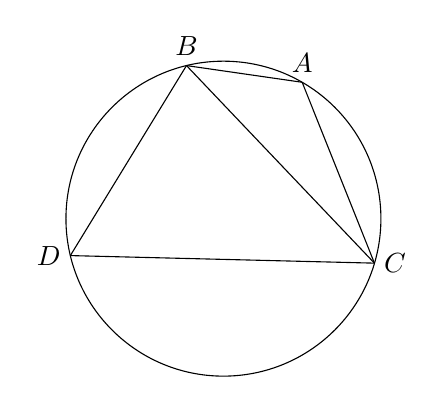
\begin{tikzpicture}
        \draw (0,0) circle (2);
        \draw (-0.469,1.944) node [above]{$B$} coordinate (B)-- (1.,1.732) node [above] {$A$} coordinate (A);
        \draw (A) -- (1.918,-0.565) node [right] {$C$} coordinate (C);
        \draw (B)-- (C);
        \draw (-1.944,-0.469) node [left] {$D$} coordinate (D)-- (C);
        \draw (B) -- (D);
    \end{tikzpicture}
\end{center}
(1) $\sin \angle BAD$的值;\\
(2) 边$BC$的长.
\item 如图, $AB$是半圆$O$的直径, 延长$AB$到$C$, 使$BC=AB$, $D$是半圆上一点, 连接$CD$, 且$\tan \angle CDB=\dfrac 13$, 求$\cos \angle DAB$的值.
\begin{center}
    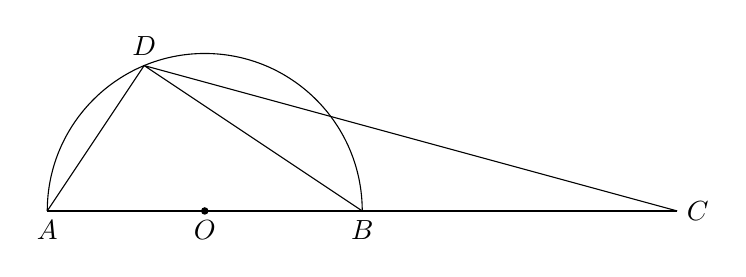
\begin{tikzpicture}[scale = 2]
        \draw (-1,0) node [below] {$A$} arc (180:0:1) node [below] {$B$};
        \draw (-0.3846,0.9231) node [above] {$D$} coordinate (D);
        \draw (-1,0) -- (D) -- (1,0) (D) -- (3,0);
        \draw (-1,0) -- (3,0) node [right] {$C$};
        \filldraw (0,0) circle (0.02) node [below] {$O$};
    \end{tikzpicture}
\end{center}
\item 已知$R,r$分別是直角三角形的外接圆半径与内切圆半径, 求$\dfrac rR$的最大值, 并说明此时三角形的形状.
\item 如图, 为了测定河的宽度, 在一岸边选定两点$A,B$, 望对岸标记物$C$, 测得$\angle CAB=30^\circ$, $\angle CBA=75^\circ$, $AB=120$米, 求河的宽度.
\begin{center}
    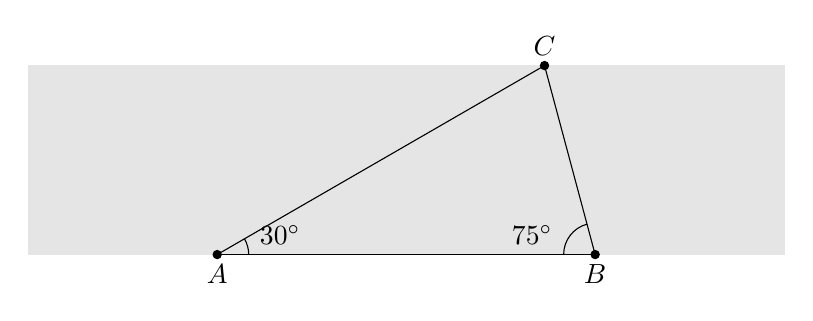
\begin{tikzpicture}[scale = 0.4]
        \filldraw [gray!20] (-6,0) rectangle (18,6);
        \draw (0,0) node [below] {$A$} coordinate (A) --++ (12,0) node [below] {$B$} coordinate (B);
        \draw ({6*sqrt(3)},6) node [above] {$C$} coordinate (C);
        \draw (A) -- (C) -- (B);
        \draw (1,0) arc (0:30:1) (2,0) node [above] {$30^\circ$};
        \draw (11,0) arc (180:105:1) (10,0) node [above]{$75^\circ$};
        \filldraw (A) circle (0.13) (B) circle (0.13) (C) circle (0.13);
    \end{tikzpicture}
\end{center}
\item 如图, 在塔底$B$测得山顶$C$的仰角为60°, 在山顶$C$测得塔顶$A$的俯角为45°, 已知塔高$AB=20$米, 求山高$DC$.
\begin{center}
    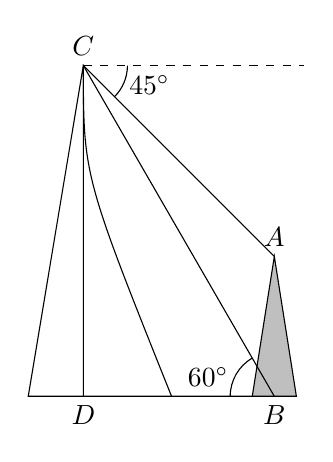
\begin{tikzpicture}[scale = 1.4]
        \draw (0,0) node [below] {$D$} coordinate (D);
        \draw ({sqrt(3)},0) node [below] {$B$} coordinate (B);
        \draw (B) ++ (0,{2*sqrt(3)/sin(135)*sin(15)}) node [above] {$A$} coordinate (A);
        \draw (D) ++ (0,3) node [above] {$C$} coordinate (C);
        \draw (A) -- (C) -- (D) -- (B);
        \draw (B) ++ (-0.2,0) coordinate (B1) (B) ++ (0.2,0) coordinate (B2);
        \filldraw [fill = gray!50, draw = black] (B1) -- (B2) -- (A) -- cycle;
        \draw (B) -- (C) -- (-0.5,0) -- (D) (C) .. controls (0,2) .. (0.8,0);
        \draw (B) ++ (-0.4,0) arc (180:120:0.4) (B) ++ (-0.6,0) node [above] {$60^\circ$};
        \draw [dashed] (C) --++ (2,0);
        \draw (C) ++ (0.4,0) arc (0:-45:0.4) (C) ++ (0.6,0) node [below] {$45^\circ$};
    \end{tikzpicture}
\end{center}
\item 如图, 半圆$O$的直径$MN$的长为2, $A$为直径延长线上一点, 且$OA=2$, $B$为半圆上任意一点, 以$AB$为边作等边$\triangle ABC$($A,B,C$顺时针排列), $\angle AOB$等于多少时, 四边形$OACB$的面积最大? 最大面积是多少?
\begin{center}
    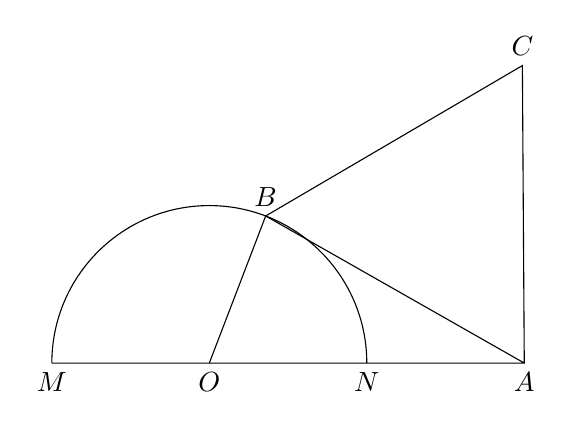
\begin{tikzpicture}[scale = 2]
        \draw (-1,0) node [below] {$M$} coordinate (M);
        \draw (1,0) node [below] {$N$} coordinate (N);
        \draw (0,0) node [below] {$O$} coordinate (O);
        \draw (2,0) node [below] {$A$} coordinate (A);
        \draw (0.358,0.934) node [above] {$B$} coordinate (B);
        \draw (1.988,1.889) node [above] {$C$} coordinate (C);
        \draw (M) -- (A) -- (C) -- (B) -- (O) (B) -- (A);
        \draw (N) arc (0:180:1);
    \end{tikzpicture}
\end{center}
\item 利用三角代换求下列函数的值域:
(1)$y=x+\sqrt {1-x^2}+3$.					(2)$y=\sqrt {x-4}+\sqrt {15-3x}$.
(3)$y=2\sqrt {x+3}+\sqrt {2-x}$.				(4)$S=x^2+xy+y^2$($1\le x^2+y^2\le 2$).
(5)$y=\sqrt {1+x}-\sqrt x$.
注意  常用的三角代换有如下几种:
若$0\le x\le 1$, 可令$x=\sin ^2\alpha$或令$x=\cos ^2\alpha$($0\le \alpha \le \dfrac{\pi}2$), 或令$x=\tan \alpha$($0\le \alpha \le \dfrac{\pi}4$);
若$-1\le x\le 1$, 可令$x=\sin \alpha$($-\dfrac{\pi}2\le \alpha \le \dfrac{\pi}2$), 或令$x=\cos \alpha$($0\le \alpha \le \pi$), 或令$x=\tan \alpha$($-\dfrac{\pi}4\le \alpha \le \dfrac{\pi}4$);
若$x^2+y^2=R^2$, 可令$x=R\cos \alpha$, $y=R\sin \alpha$($0\le \alpha \le 2\pi$);
若$x\in \mathbf{R}$, 可令$x=\tan \alpha$($-\dfrac{\pi}2<\alpha <\dfrac{\pi}2$);
若$x^2-y^2=1$, 可令$x=\sec \alpha$, $y=\tan \alpha$($0\le \alpha <\dfrac{\pi}2$)
\item (1.)求函数$f(x)=\sqrt {x-1}+\sqrt {2-x}$的最大值、最小值.
(2)已知$a,b>0$, 求函数$f(x)=a\sqrt {1-x^2}+bx$的最大值、最小值.
(3)已知$0\le y<x<\dfrac{\pi}2$, 且满足$\tan x=3\tan y$, 求$x-y$的最大值.
\item (1)$0<\alpha <\beta <\dfrac{\pi}2$, 且$\sin \alpha$, $\sin \beta$是方程$x^2-(\sqrt 2\cos 40^\circ)x+\cos ^240^\circ -\dfrac 12=0$的两根, 求$\cos (2\alpha -\beta)$的值.
(2)在$\triangle ABC$中, $\tan A$, $\tan B$是关于$x$的二次方程$x^2+mx+m+1=0$的两个实根, 求实数$m$的取值范围.
\item 如图, 已知$P$为$\triangle ABC$内一点, 且满足$\angle PAB=\angle PBC=\angle PCA=\theta$, 求证: $\cot \theta =\cot A+\cot B+\cot C$.
\begin{center}
    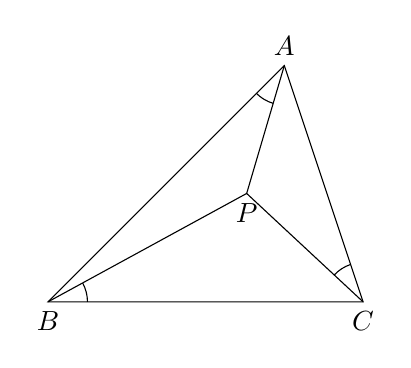
\begin{tikzpicture}
        \draw (-2,0) node [below] {$B$} coordinate (B);
        \draw (2,0) node [below] {$C$} coordinate (C);
        \draw (1,3) node [above] {$A$} coordinate (A);
        \draw (0.522,1.376) node [below] {$P$} coordinate (P);
        \draw (A) -- (B) -- (C) -- cycle;
        \draw (A) -- (P) -- (B) (P) -- (C);
        \pic (A) [draw] {angle = B--A--P};
        \pic (B) [draw] {angle = C--B--P}; 
        \pic (C) [draw] {angle = A--C--P};
    \end{tikzpicture}
\end{center}
\item 若不等式$\dfrac{(x^2+1)\cos \theta -x(\cos \theta -5)+3}{x^2-x+1}>\sin \theta -1$对任意实数$x$恒成立, 求$\theta$的取值范围.
\item 已知函数$f(x)=a+b\cos x+c\sin x$的图像过两点(0, 1), $(\dfrac{\pi}2,1)$, 且当$x\in [0,\dfrac{\pi}2]$时, $|f(x)|\le 2$, 求实数$a$的取值范围.
\item (1)已知$\odot O$的半径为$R$, 它的内接三角形$ABC$满足关系式$2R(\sin ^2A-\sin ^2C)=(\sqrt 2a-b)\sin B$, 求$\triangle ABC$面积的最大值.
(2)如图, 已知扇形$AOB$的中心角为45°, 半径为1, 矩形$MNPQ$内接于扇形, 使$P,Q$点在半径$OA$上, 求矩形$MNPQ$的对角线$PM$的最小值.
\begin{center}
    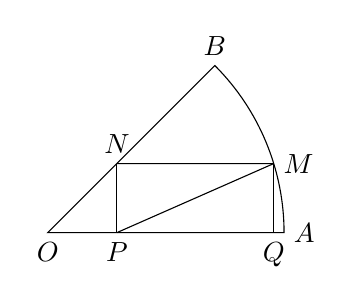
\begin{tikzpicture}[scale = 3]
        \draw (0,0) node [below] {$O$} coordinate (O) -- (1,0) node [right] {$A$} coordinate (A) arc (0:45:1) node [above] {$B$} coordinate (B) -- cycle;
        \draw (17:1) node [right] {$M$} coordinate (M);
        \path [name path = MN] (M) --++ (-0.7,0);
        \path [name path = OB] (O) -- (B);
        \path [name intersections = {of = MN and OB, by = N}];
        \draw (M) -- (N) node [above] {$N$};
        \draw ($(O)!(N)!(A)$) node [below] {$P$} coordinate (P) -- (N);
        \draw ($(O)!(M)!(A)$) node [below] {$Q$} -- (M);
        \draw (P) -- (M);
    \end{tikzpicture}
\end{center}
(3)如图, 已知$P$是正方形$ABCD$内一点, $PQ\perp BC$, $PR\perp CD$, ($Q,R$为垂足), $AB=10$, $AP=9$, 求矩形面积的最大值、最小值.
\begin{center}
    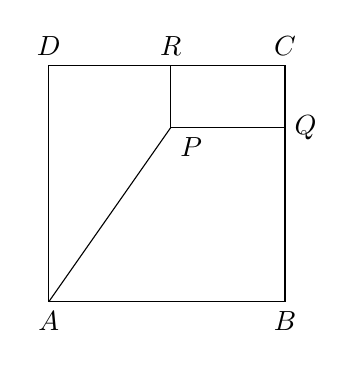
\begin{tikzpicture}[scale = 0.3]
        \draw (0,0) node [below] {$A$} coordinate (A);
        \draw (10,0) node [below] {$B$} coordinate (B);
        \draw (10,10) node [above] {$C$} coordinate (C);
        \draw (0,10) node [above] {$D$} coordinate (D);
        \draw (A) -- (B) -- (C) -- (D) -- cycle;
        \draw (55:9) node [below right] {$P$} coordinate (P) -- (A);
        \draw ($(C)!(P)!(D)$) node [above] {$R$} -- (P);
        \draw ($(C)!(P)!(B)$) node [right] {$Q$} -- (P);
    \end{tikzpicture}
\end{center}
\item (1)若$x\ne k\pi$($k\in \mathbf{N}$), 求证:
\textcircled{1} $\dfrac 1{\sin 2x}=\cot x-\cot 2x$;
\textcircled{2} $\dfrac 1{\sin 2x}+\dfrac 1{\sin 2^2x}+\cdots +\dfrac 1{\sin 2^nx}=\cot x-\cot 2^nx$.
(2)求证: $\tan x\tan 2x+\tan 2x\tan 3x+\cdots +\tan (n-1)x\tan nx=\dfrac{\tan nx}{\tan x}-n$($n\in \mathbf{N}$).
(3)求证: $(2\cos \theta -1)(2\cos 2\theta -1)(2\cos 2^2\theta -1)\cdot \cdots \cdot (2\cos 2^{n-1}\theta -1)=\dfrac{2\cos 2^n\theta +1}{2\cos \theta +1}$
\item 求$\cos \dfrac{\pi}{17}\cos \dfrac{2\pi}{17}\cos \dfrac{3\pi}{17}\cos \dfrac{4\pi}{17}\cos \dfrac{5\pi}{17}\cos \dfrac{6\pi}{17}\cos \dfrac{7\pi}{17}\cos \dfrac{8\pi}{17}$的值.
\item 实数$x,y,z$满足$\sin x=a\sin (y-z)$, $\sin y=b\sin (z-x)$, $\sin z=c\sin (x-y)$($a,b,c\ne 1$), 且$\sin (x-y)$, $\sin (y-z)$, $\sin (z-x)$都不为$0$, 求$a,b,c$应满足的关系式.
    
    
\end{enumerate}
\end{document}